\documentclass{article}
% \documentclass[review]{elsarticle}
\usepackage{epsfig}
\usepackage{amsmath}
\usepackage{mathtools}
\usepackage{algorithm}
\usepackage[algo2e,noend]{algorithm2e}
\usepackage[compatible,noend]{algpseudocode}
\usepackage{enumitem}
\usepackage{xspace}
\usepackage[table,xcdraw]{xcolor}
\usepackage{amsfonts}
\usepackage{pifont}
\usepackage{bbding}
\usepackage[english]{babel}
\usepackage{adjustbox}
\usepackage{tikz}
\usepackage{subcaption}
\usetikzlibrary{automata, topaths, calc, positioning, shapes, backgrounds, fit, matrix}
\usepackage{caption}
\usepackage{tabularx}
\usepackage[T1]{fontenc}
\usepackage{graphicx}
\usepackage{natbib}
\usepackage{datatool}
\usepackage{array}
\usepackage{pgfplotstable}
\pgfplotsset{width=7cm,compat=newest}
\usepackage{booktabs}
\usepackage{longtable}
\usepackage{pdflscape}
\usepackage{afterpage}
\usepackage{capt-of}
\usepackage{multirow}
\usepackage{float}
\usepackage[text={15cm,21cm},centering]{geometry}
\usepackage{setspace}
\usepackage{array}
\allowdisplaybreaks
\usepackage{lineno}
\usepackage{tkz-graph}
\usepackage{breqn}

\tikzset{
base/.style = {shape=rectangle, 
                      anchor=center,minimum size=5mm, 
                     align=center,
                     top color=white, ,inner sep=0ex,
                     minimum size=5mm
                     },
    LC11/.style =   {  base,   
                    text width=3em, 
                    bottom color=brown!100,
                    },
    UC11/.style = {     base,    
                    text width=5em, 
                    bottom color=brown!100,
                    align = right,
                },
    LC12/.style =   {  base,   
                    text width=1em, 
                    bottom color=orange!100,
                    },
    UC12/.style = {     base,    
                    text width=2.5em, 
                    bottom color=orange!100,
                },
    LC21/.style =   {  base,   
                    text width=1.5em, 
                    bottom color=brown!100,
                    },
    UC21/.style = {     base,    
                    text width=3.5em, 
                    bottom color=brown!100,
                },
    LC22/.style =   {  base,   
                    text width=4em, 
                    bottom color=blue!100,
                    },
    UC22/.style = {     base,    
                    text width=7em, 
                    bottom color=blue!100,
                    align = left,
                },
    UC221/.style = {     base,    
                    text width=3.5em, 
                    bottom color=blue!100,
                    % color=blue!100,
                    outer xsep=0em,
                    % align = right,
                },
                UC231/.style =   {  base,   
                    text width=1.5em, 
                    bottom color=blue!100,
                    },
    LC23/.style =   {  base,   
                    text width=1.5em, 
                    bottom color=orange!100,
                    },
    UC23/.style = {     base,    
                    text width=2.em, 
                    bottom color=orange!100,
                },
  env/.style      = {base, font=\ttfamily\normalsize},
label/.style   = {base,font=\ttfamily\normalsize, text width = 8em, 
  inner sep=0em, rounded corners=1mm,bottom color=red!80,},
  dummy/.style    = {circle,draw}
}
\newcolumntype{H}{>{\setbox0=\hbox\bgroup}c<{\egroup}@{}}

\newtheorem{theorem}{Theorem}[section]
\newtheorem{lemma}[theorem]{Lemma}
\newtheorem{proposition}[theorem]{Proposition}
\newtheorem{corollary}[theorem]{Corollary}
\newtheorem{definition}[theorem]{Definition}
\newcommand{\pcmaxc}{P$|\mbox{\em cont}|$C$_{\max}$\xspace}

\newcommand{\GRASP}{Greedy randomized adaptive search procedure\xspace}
\newcommand{\F}{$\mathcal{F}$\xspace}
\newcommand{\B}{$\mathcal{B}$\xspace}
\newcommand{\C}{$\mathcal{C}$\xspace}
\newcommand{\LB}{$\mathcal{L}$\xspace}
\newcommand{\Lb}{$\mathcal{L}_b$\xspace}
\newcommand{\D}{$\mathcal{D}$\xspace}
 \newcommand*{\red}{\textcolor{red}}

\renewcommand{\algorithmicforall}{\textbf{for each}}
\SetKwFor{ForEach}{for each}{}{}%
\renewcommand{\algorithmiccomment}[2][1\linewidth]{%
\leavevmode\hfill\makebox[#1][l]{/* \textbf{~#2} */}}
\renewcommand{\algorithmicrequire}{\textbf{Input:}}

\renewcommand{\tabcolsep}{4pt}

\modulolinenumbers[1]
\linenumbers

\oddsidemargin=0.5in
\topmargin=-0.25in
\textwidth=5.5in
\textheight=8.25in

%\journal{European Journal of Operational Research}

%\begin{frontmatter}

		
\title{A GRASP algorithm for the concrete delivery problem. }
\author{Ousmane Ali$^{(1)}$, Jean-Fran\c cois C\^ot\'e$^{(2)}$, Leandro C.~Coelho$^{(3)}$\\
 $(1)$ {\tt nassoma-wattara-ousmane.ali.1@ulaval.ca}\\
 $(2)$ {\tt Jean-Francois.Cote@fsa.ulaval.ca}\\
 $(3)$ {\tt Leandro.Coelho@fsa.ulaval.ca}\\
}

% \date{\today}

\begin{document}
\maketitle
\begin{abstract}
    This paper addresses a novel variant of the Concrete Delivery Problem (CDP), which involves the efficient scheduling of ready-mixed concrete deliveries to construction sites while balancing the conflicting goals of minimizing transportation costs and maximizing customer satisfaction. In this study, we propose an exact formulation and a heuristic approach based on the Greedy Randomized Adaptive Search Procedure (GRASP), to tackle this challenging CDP variant. This variant introduces realistic side constraints, including driver working shifts, a minimum driver working time, and overtime penalties. Additionally, it considers the scenario where customers may request multiple types of concrete delivered within the same time window. We assess the performance of our heuristic using new public instances generated for this problem and provide a comparative analysis with another CDP variant to demonstrate its effectiveness.
\end{abstract}



% \begin{keywords}
\noindent{\textbf{Keywords:} Vehicle scheduling;  concrete delivery; GRASP; ready-mixed concrete }
% \end{keywords}

%\end{frontmatter}

\section{Introduction}
\label{sec:intro}
Concrete is a widely used building material in construction projects. Its perishable nature is affected by many factors that impact its quality \citep{sinha_quality_2021}, which is crucial for the durability and strength of the final construction. Concrete comes in two types: ready-mixed concrete (RMC) and site-mixed concrete (SMC). RMC is manufactured in a batch plant and delivered to the construction site, while SMC is produced on-site using raw materials stored on the construction site. Using SMC can avoid delays caused by road traffic, but it has a slower and more difficult production process, requires storage for mixing materials and equipment, and is suitable for low amounts of concrete. On the other hand, RMC has better quality and benefits from lower production costs \citep{muresan_comparing}. However, to take advantage of these benefits, the batch plant manager must ensure efficient and prompt delivery on the construction site, which may require a fleet of high-cost revolving drum trucks (concrete mixers) to dispatch the RMC.

Concrete delivery under the form of RMC is subject to many operational constraints that make the Concrete Delivery Problem (CDP) very challenging. In this paper, we study a variant of the CDP to schedule the daily production and dispatching of RMC for a company located in the province of Quebec, Canada. This company operates multiple batch plants with varying production rates, using a fleet of concrete mixers of different capacities. Each plant has its own fleet of trucks; however, under certain conditions, the trucks can move between plants if necessary. The trucks must return to their home plant at the end of the day. The company owns two types of trucks with different capacities and can call on an external fleet when needed. They serve construction sites from any of their plants, with the first delivery starting at the time specified by the customer. The loading and unloading of a concrete mixer depend on the truck capacity, the loading rate at the plant, and the unloading rate at the construction site. Drivers are allocated based on their daily work schedules. A customer may request several types of concrete to be delivered within the same time window, with no required sequence for the orders, but an order can only start after the completion of the previous order. This constraint generalizes the linked order constraints of \cite{durbin2008or} where some customers place two orders for the same day and request that they are linked (the second order begins only after the first order is completed). The setting of our study is similar to a variant of the CDP previously studied in \cite{schmid2009hybrid, schmid2010hybridization}. However, we include the plant's production rate and driver shift schedule. The company uses a centralized dispatcher system to schedule all daily orders, but this system has issues satisfying all daily demands without using an external fleet or using different plants to serve the same order.
% Also, as per union rules, they assign a truck driver to a delivery task based on his seniority.

According to \cite{blazewicz2019handbook}, the CDP combines vehicle routing with scheduling issues to plan routes to deliver concrete from batch plants (depots) to customers' construction sites. RMC is an on-demand product with a short life cycle from production through end use. It cannot be stored and cannot stay too long on a truck, or it will harden. Hence, concrete mixers must deliver RMC at the planned construction site shortly after its production. \cite{tommelein1999just} describes RMC production and delivery as an example of a just-in-time (JIT) production system in construction. A customer quantity requirement is often greater than the truck size and must be fulfilled by multiple deliveries. In that sense, CDP is similar to the vehicle routing problem with split delivery \citep{archetti2008split}, except that the same truck may visit a customer more than once. Concrete hardens quickly, so multiple deliveries must be done back-to-back or at least close in time to avoid the problem of cold joint, which can reduce the strength and durability of the concrete. Customers request to be served within a specific time window, which can complicate truck-loading schedules when a plant can only load one truck at a time. Similarly, only one truck can unload at a time at a customer location, sometimes leading to concrete mixers queuing and waiting their turn to deliver. Furthermore, with trucks of varied sizes, loading, travel, and unloading times that may be uncertain, the CDP is a complex and challenging problem.

In this paper, we propose a mathematical model and a Greedy Randomized Search Procedure (GRASP) heuristic to solve a new variant of the CDP. Our model takes into consideration the working shifts of the drivers and the scheduling of multiple orders within the same time window at a construction site. To the best of our knowledge, this paper is the first that deals with these specific constraints in the context of the CDP.

The rest of the paper is organized as follows: Section \ref{lit_review} provides a literature review of previous work related to the CDP. Section \ref{desc_form} provides a formal description and mathematical model of the problem. Section \ref{grasp_method} describes the GRASP algorithm and the constructive heuristics developed to solve this variant of the CDP. Section \ref{comp_exp} presents computational experiments and sensitivity analyses to evaluate the proposed approach, and finally, section \ref{concl} presents the conclusions.

\section{Literature review}
\label{lit_review}

Academic Research on concrete batch and delivery began in the late 1990s. \cite{tommelein1999just} described RMC as a prototypical example of a JIT production system in construction and identified two practices for delivering it. One approach is for the customer to haul the product from the batch plant with their concrete mixer, while the other is for the batch plant to deliver the concrete directly to the customer's location. This latter approach is the one that has been studied in all related papers found in the literature. Several works to schedule and dispatch concrete production and delivery have mainly focused on simulation-related methods. These methods can be standalone, such as those used by \cite{zayed2001simulation, wang2001scheduling, tian_simulation_based_2010, panas_simulation_based_2013} and \cite{galic2016simulation}, among others. Alternatively, these methods can be hybridized with optimization techniques, such as those used by \cite{feng2004optimizing, lu2005optimized}, and \cite{feng_integrating_2006}. \cite{wang2001scheduling} developed a simulation model to reveal the effect and value of the concrete mixers' inter-arrival time on the productivity of hired unloading equipment on site. \cite{feng2004optimizing} used a combination of genetic algorithm (GA) and simulation process to minimize the total waiting time for trucks at a customer site. The study focused on loading trucks with identical capacities at the same batch plant, with fixed loading and unloading durations. The GA was used to find the best loading sequence of RMC trucks to be assigned to different construction sites. The simulation process determined the loading, arrival, departure, and waiting time of trucks and thus evaluated the cost of each dispatching sequence. They evaluated their method using data from a batch plant in Taiwan with up to nine customers served. \cite{mayteekrieangkrai2015optimized} addressed the same problem with the same data using a bee algorithm (BA) and found better solutions than the GA. \cite{lu2005optimized} used the same combination of GA and simulation to determine the optimal number of concrete mixers to be deployed and an optimal schedule for batching and delivering concrete. Their objective was to minimize the idle time of the site crew due to late concrete deliveries and truck queuing time. In this setting, it was also necessary to deliver a batch of mortar on-site to lubricate the unloading pump before the concrete delivery. As such, the simulation model also included the batch and delivery of mortar. Finding the best RMC fleet size was also the purpose of the discrete-event simulation model proposed by \cite{panas_simulation_based_2013}.

In addition to simulation-based methods, several other approaches have been used in the literature to solve the CDP. These include metaheuristics \citep{faria2006distributed, misir2011selection, maghrebi2016sequential, yang2022concrete}, exact methods \citep{yan2007optimal, asbach2009analysis, kinable2014concrete}, matheuristics \citep{schmid2009hybrid, schmid2010hybridization}, Benders Decomposition \citep{maghrebi2014benders}, column generation (CG) \citep{maghrebi2014solving, maghrebi2016column}, Lagrangian relaxation \citep{narayanan2015using}, and machine learning approaches such as those used by \cite{graham2006modeling, maghrebi2014exploring, maghrebi2016matching}. \cite{matsatsinis2004towards} designed a decision support system (DSS) for the dynamic routing of both concrete and pumps that may be necessary for some construction sites to aid in the unloading of concrete. The DSS considered the availability of three plants but stipulated that vehicles fulfilling the same order must all load at the same plant. Orders that could not be executed immediately could be postponed for the next day. The routing of the pumps was modeled as a multi-depot vehicle routing problem with time windows. \cite{naso2007genetic} proposed a sequential GA method combined with constructive heuristics to solve another variant of the CDP. In this problem, the plant's production schedule must account for orders for concrete to be delivered to a customer site and orders that customers must pick up themselves. The algorithm first schedules the plant loading operations before scheduling truck deliveries. The authors also developed a non-linear model that minimizes transportation costs, waiting times, outsourced costs, and overtime work. They ran experiments using real-world instances of a concrete supply chain in the Netherlands and found a reduction in the number of outsourced requests. \cite{yan2007optimal} also considered overtime considerations in their paper, which focused on scheduling RMC for one batch plant with two loading docks. The study took into account that overtime wages are paid for factory and construction site operations after 4 PM. They developed a mixed-integer programming (MIP) model on a time-space network to minimize travel times and operating costs at both normal and overtime working hours at the plant and the construction sites. They tested the model using real data consisting of three days of operation using a two-stage algorithm. First, they solved the MIP relaxation with CPLEX. Then, they simplified the original model by fixing some decision variables before solving it. The algorithm was found to improve the actual plant operation by 10\%. A time-space network is the key component of the real-time DSS developed by \cite{durbin2008or} to solve a dynamic CDP every five minutes. The DSS can receive new orders, schedule them on the fly, and handle unexpected events such as plant closures, truck breakdowns, and delays in transportation times. The authors combined the DSS with a tabu search (TS) heuristic to warm start CPLEX, which made the model performant enough to solve instances with up to 1,500 loads per day with up to 250 trucks. The DSS also considers the case of a customer who places two orders, with the first being completed before the second starts. Further insights on the real-time planning and monitoring of CDP are available in \cite{garza2021dynamic}. Another variant of the CDP is modeled by \cite{schmid2009hybrid} as an integer multicommodity network flow (MCNF) problem on a time-space network. In this paper, concrete is delivered using a heterogeneous fleet of vehicles, and each plant can load an unlimited number of trucks simultaneously. Some of the trucks have specialized equipment and must arrive first at certain construction sites to assist in unloading the concrete. The objective is to fulfill all orders, minimize the travel cost, and avoid delays between two consecutive unloading operations for an order. The model is typically solved using a matheuristic algorithm that combines the MCNF with a variable neighborhood search (VNS) heuristic. The method can quickly solve large problem instances with more than 60 orders per day without encountering any memory issues. The same problem is addressed by \cite{schmid2010hybridization}, who proposed a MIP model combined with a VNS and a very large neighborhood search (VLNS) to develop two matheuristics approaches. Comparisons between both matheuristics and a standalone VNS show that the former methods are much better and suitable for solving larger problem instances. These methods also provide better solutions for small to medium instances than the matheuristic used in \cite{schmid2009hybrid}. A pure VNS approach with the same problem but without the use of instrumentation has been applied by \cite{payr2009optimizing}.

Regarding objectives, most authors have focused on minimizing travel time and delays between consecutive deliveries. However, some authors have been more interested in maximizing customer satisfaction alone. We find these situations in the works of \cite{durbin2008or, kinable2014concrete, kinable2014logic, sulaman2017simulated}. \cite{kinable2014concrete} introduce a general MIP and constraint programming (CP) models of the CDP reflecting the main constraints commonly found in all CDP works: time lag and no overlapping between consecutive deliveries, covering of all customers' demands, delivery time window, and heterogeneous fleet. However, the model did not include constraints limiting the time that concrete may reside in a truck. The authors propose a constructive heuristic that schedules the visits to the customers one by one according to the start time of the visit and the truck capacity. The procedure is invoked multiple times for different permutations of the customer's order which is determined using the steepest descent (SD) local search procedure. One of the paper's main contributions is the creation of the first public test instances for the CDP with up to 50 customers, four batch plants, and 20 concrete mixers. They found the CP model to be highly effective in finding high-quality solutions in a relatively short time or improving existing schedules, while the MIP model can be used to compute bounds, as it seems ineffective in solving large problem instances. Finally, the heuristic often yields good solutions in less than a second. A detailed analysis of the MIP model presented in \cite{kinable2014concrete} and of two more compact models can be found in the thesis of \cite{hernandez_lopez_study_2020}. In \cite{kinable2014logic}, we found an attempt to solve the previous problem with a logic-based Benders' approach. %\cite{sulaman2017simulated} expand upon the SD-heuristic proposed in \cite{kinable2014concrete}, proposing a simulated annealing (SA) combined with a time-slot Heuristic (SATH). This method looks for a slot between existing visits of a truck to schedule a new delivery instead of assigning it to the time slot strictly after the truck's latest assigned delivery. The goal is to reduce the large time gaps that can be present in a schedule created with SD due to ignoring the intermediate available time slots. Experimental results indicated that SATH outperforms SD in speed and solution quality. 
A generalization of the MIP model of \cite{kinable2014concrete} is addressed in \cite{asbach2009analysis}. This model simultaneously minimizes the total sum of travel costs and the penalty costs for customers with unfulfilled demand. A customer can request that all concrete deliveries come from the same plant or a subset of plants and that a delivery truck belongs to a subset of the vehicle fleet. The MIP model is used in a local search scheme as a black-box solver to reoptimize an incumbent solution in which a neighborhood operator has unfixed some variables. \cite{tzanetos2023systematic} provide an overview of the various methods used in the literature to address the CDP and categorizes the problem formulations based on the different concepts used in the literature. They also discussed the consistency between industry needs and existing constraints and provided insights into the datasets corresponding to real-world cases, identifying the necessary data for practitioners.

\section{Problem description}
\label{desc_form}
The focus of this paper is on the distribution of RMC from a Canadian company that operates in the greater Montreal area. When a customer places an order, it is received at a control center and immediately assigned to one of the company's batch plants. These plants produce the concrete and then deliver it to the customer. The problem we are examining involves a set of customer orders, a set of concrete-mixer drivers, and a set of batch plants.

% \subsection*{Customer orders}

A customer $i$ requests one or more types of concrete to be delivered to their construction site on a specific day, with the delivery service starting at the due time $a_i$.  We call an order $o$ a request for a specific type of concrete. $q_i$ is the sum of the demands $q_o$ of each order $o$ placed, $a_i$ is the desired arrival time of the first concrete mixer, and $\tau^u_i$ is the unloading rate for customer $i$. If the order requires more concrete than a single truck can carry, multiple deliveries are scheduled. We will accept a first delivery if it arrives within a time window of $\left[a_i, a_i + \tau^w \right]$, where $\tau^w_i$ is a user-defined parameter.

Let $O_i$ be the set of all orders requested by customer $i$. Each element of $O_i$ must be fully delivered before moving on to another order. Exactly one order $o \in O_i$ must have its first delivery start at $a_i$, while the others can start at most $\gamma^2$ time after $o$ is completed. A plant is assigned to an order, and it must be the supplier of all subsequent deliveries of that order.
To avoid cold joint problems with the concrete, subsequent deliveries of the same order must be made in close succession. We define a maximum time delay $\gamma^1$ after which no more deliveries are allowed. The customer's unloading rate and the quantity to be unloaded give the time required to unload a truckload. Let $\mathcal{C}$ be the set of construction sites (customers) with a planned delivery for the day, and $\mathcal{O}=\{{O_i, i \in \mathcal{C}}\}$ be the set of all requested orders for all customers.

% \subsection*{Drivers}

The company has two types of concrete mixer trucks with capacities of 8 and 12 cubic meters. Each driver $k$ is assigned to a particular batch plant and is responsible for driving a truck with capacity $Q_k$. The set of drivers is represented by $K =\cup_{b \in \mathcal{B}}K_b $, where $K_b$ is the set of drivers scheduled to start their shift at batch plant $b$. $t_{ij}$ is the known time to travel between any two locations $i$ and $j$. A scheduled driver $k$ is required to start his shift at $H_k$, work a minimum of $M_T$ hours and a maximum of $N_T$ hours during regular working hours, with the possibility of overtime of up to $O_T$ hours. $\beta_3$ and $\beta_4$ are the penalties for a driver working less than $M_T$ and more than $N_T$.

A driver typically loads RMC at his assigned batch plant but may be required to drive to and load at other plants if needed. The batch plant produces concrete on demand using recipes specific to each order. This means that a truck can only haul RMC for one order, even if there is spare capacity.  After unloading the RMC,  driver $k$ takes $\rho$ minutes to clean the concrete mixer before proceeding. %When assigning drivers to deliveries, the company prioritizes employees with the highest seniority.

Let $n_o$ be the number of deliveries needed to fulfill the order $o$. $n_o$ is not known in advance because we use a fleet of trucks with different capacities. However, we can compute its lower ($n_o^{min}$) and upper ($n_o^{max}$) bounds using the capacities of the largest ($Q_{max}$) and smallest ($Q_{min}$) available trucks.
\begin{alignat}{3}
    \label{mod:c0}
    n_o^{min} = \left\lceil \frac{q_o}{Q_{max}} \right\rceil \leq n_o \leq n_o^{max} = \left\lceil \frac{q_o}{Q_{min}} \right\rceil & \text{ } &
    \forall  o \in \mathcal{O}.
\end{alignat}

Let $d^j_{o}$ be the $j^{th}$ visit with load $q^j_{o}$ for order $o$. We represent the fulfillment of order $o$ by the visits to the ordered set of delivery nodes $\mathcal{D}_o= \left(d^0_{o},d^1_{o},\cdots, d^{n_o}_{o}\right)$. The deliveries of customer $i$ are the ordered set $\mathcal{D}_i= (\mathcal{D}_{o_1}, \mathcal{D}_{o_2},\cdots,\mathcal{D}_{o_{|O_i|}})$, where $o_r$ is the $r^{th}$ delivered order. We will refer to $d \in \mathcal{D}_i$ ($d \in \mathcal{D}_o$) as the $d^{th}$ potential delivery of customer $i$ (order $o$). $\mathcal{D}=\bigcup_{i\in \mathcal{C}} \mathcal{D}_i$ is the union of all delivery nodes.

% \subsection*{Batching plants}

Each of the company's plants has a single loading dock that can accommodate only one truck at a time. As a result, trucks often form a queue while waiting for their turn at the loading dock. Let $\mathcal{B}$ be the set of batch plants. The plants are heterogeneous, as each plant $b$ has its hourly loading rate, represented by $\tau^l_b$, which affects the duration of the loading process. After loading the concrete, the driver spends $\alpha_b$ minutes adjusting the concrete in the truck before heading to the customer site. Each plant has its own assigned fleet of trucks, but it can borrow trucks from other plants. Let $l_{j}$ be the loading dock node associated with delivery node $j$. After loading RMC at $l_j$, it must be fully delivered to $j$ at most before $\Delta$ time, which is the concrete lifetime. We denote $\mathcal{L}_b$ as the set of loading dock nodes of plant $b$ and $\mathcal{L}$ as the set of all loading docks.

% \subsection*{Model}
A solution to the problem involves decisions about truck loading schedules, driver assignments to different deliveries, and truck arrival times at construction sites for unloading. For a batch plant, the decision involves choosing which driver to load, when to load them, how much to load, and which construction site to deliver. For a driver, the decision is to determine the sequence of loading depots and delivery sites. And for a construction site, the decision involves determining the arrival times of all scheduled deliveries for the day.

Each driver leaves and returns to their home plant every day. We represent the home plant of a driver $k$ with a starting depot $s_k$ and an ending depot $e_k$. $S$ and $E$ are the sets of starting and ending depots, respectively.

We define our problem on a complete directed graph where $V=\{ S \cup \mathcal{L} \cup \mathcal{D} \cup E\}$ is the set of nodes. The arc sets are $A =  \{(i,j,k) \hspace*{1mm} \vert \hspace*{1mm} i, j \in V \hspace{1mm} k\in K \}$, $A^D = \{(i,j) \hspace*{1mm} \vert \hspace*{1mm} i, j \in \mathcal{D} \hspace{1mm} \}$, and $A^L = \{(i,j) \hspace*{1mm} \vert \hspace*{1mm} i, j \in \mathcal{L} \hspace{1mm} \}$.
$A$ corresponds to allowed movements of drivers from node $i$ to node $j$. For each driver $k$, the allowed movements are the following:

\begin{itemize}
    \item From the starting depot $s_k$ to a loading dock $l \in \mathcal{L}$ or to the ending depot $e_k$.
    \item From a loading dock $l \in \mathcal{L}$ to a delivery node $d \in \mathcal{D}$.
    \item From a delivery node  $d \in \mathcal{D}$ to a loading dock $l \in \mathcal{L}$ or to the ending depot $e_k$.
\end{itemize}

For a customer $c$, arcs in $A^D$ link consecutive delivery nodes of the same order   $\lbrace (i,j)\in \mathcal{D}_o, o \in \mathcal{O}_c, i < j  \rbrace$, and pair of delivery nodes of two different orders $ \lbrace (i,d^{0}_{o_2}),  i \in \mathcal{D}_{o_1}, i \geq n^{min}_{o_1}, o_1, o_2 \in \mathcal{O}_c, o_1 \neq o_2 \rbrace $. Arcs in $A^L$ link all pairs of loading docks of the same batch plant.

We define $\delta^{+}(i) = \{(i, j,k) \in A \}$ and $\delta^{-}(i) = \{(j, i,k) \in A \}$ as the outcoming and incoming arc sets of node $i \in V$; $\delta^{+}_D(i) = \{(i, j)  \in A^D\}$ and $\delta^{-}_D(i) = \{(j, i) \in A^D \}$ are the outcoming and incoming arc sets of delivery node $i \in \mathcal{D}$.  Similarly, $\delta^{+}_L(i) = \{(i, j)  \in A^L\}$ and $\delta^{-}_L(i) = \{(j, i) \in A^L \}$ are the outcoming and incoming arc sets of loading node $i \in \mathcal{L}$.

Let the binary variable $x^{k}_{ij}$ be $1$ if driver $k$ travels from node $i$ to $j$. Binary variable $y_o$ is $1$ when order $o$ is completely served; $v_i$ and $w_i$ are the start and end of the loading (unloading) operation at node $i \in \mathcal{L}\cup \mathcal{D}$. Binary variable $u_{ij}$ is $1$ if node $j$ is served just after $i$, the service being either an unloading or a loading operation. % Binary variable $\sigma_{ib}$ is equal to 1 if the orders of customer $i$ are loaded by plant $b$. 
Variable $q^k_j$ is the quantity to be loaded towards $j$ with vehicle $k$. Let $w^1_k$ be a continuous variable indicating the difference between the driver's work time and the minimum number of hours to be worked in a day, and $w^2_k$ indicating the difference between the driver's work time and the normal work time. Let $g_i$ be the time between the due date and the first service start for customer $i$.

The objective function minimizes total travel cost ($TC$), penalties associated with unfulfilled orders, first delivery delays ($FDD$), driver underutilization costs ($DUC$), and driver overtime costs ($DOC$). Together, these components drive the optimization process to find a solution that efficiently balances travel costs, customer satisfaction, on-time delivery, driver utilization, and scheduling constraints.

\begin{alignat}{3}
    \label{mod:obj}   \min & \smashoperator{ \sum_{ \substack{(i,j,k) \in A} }} {t_{ij}x^{k}_{ij}} + \beta_1\smashoperator{\sum_{ o \in \mathcal{O}}}{  \left(1-y_o\right)} \hspace{-0mm}  + \beta_2 \smashoperator{ \sum_{i \in \mathcal{C} } } { g_i  } +  \sum_{k \in K}\left({\beta_3 w^{1}_k  + \beta_4  w^{2}_k}\right) &                                                                                                  \\
    \label{mod:c1}         & \sum_{j \in \delta^{+}(i) }{x^k_{ij}} =1                                                                                                                                                                                                                                                         & \forall i \in S, k \in K                                                                         \\
    \label{mod:c2}         & \sum_{j \in \delta^{-}(i)}{x^k_{ji}} = 1                                                                                                                                                                                                                                                         & \forall i \in E, k \in K                                                                         \\
    \label{mod:c03}        & v_j \geq  w_i  - M\left(1-x^{k}_{ij}\right)                                                                                                                                                                                                                                                      & \hspace{-20mm}  i \in S, j \in \delta^{+}(i),  k \in K                                           \\
    \label{mod:c3}         & v_j \geq  w_i + \alpha_{b} + t_{ij} - M\left(1-x^{k}_{ij}\right)                                                                                                                                                                                                                                 & \hspace{-20mm} \forall b \in \mathcal{B}, i \in \mathcal{L}_b, j \in \delta^{+}(i),  k \in K     \\
    \label{mod:c4}         & v_j \geq  w_i + \rho + t_{ij} - M\left(1-x^{k}_{ij}\right)                                                                                                                                                                                                                                       & \hspace{-20mm} \forall i \in \mathcal{D}  , j \in \delta^{+}(i), k \in K                         \\
    \label{mod:c5}         & w_{i} \geq v_{i}  + \frac{q^k_j}{\tau^l_b} -M\left(1- x^{k}_{ij}\right)                                                                                                                                                                                                                          & \hspace{-20mm} \forall  b \in \mathcal{B},  i \in \mathcal{L}_{b},  j \in \delta^{+}(i), k \in K \\
    \label{mod:c6}         & w_{j} \geq v_{j}  + {  \frac{q^k_j}{\tau^u_c} -M\left(1- x^{k}_{ij}\right) }                                                                                                                                                                                                                     & \hspace{-20mm}  \forall c \in  \mathcal{C}, j \in \mathcal{D}_{c}, i \in \delta^{-}(j),  k \in K \\
    \label{mod:c7}         & w_{j} \leq v_{i}  + \Delta + M\left(1- x^{k}_{ij}\right)                                                                                                                                                                                                                                         & \hspace{-20mm}   j \in \mathcal{D},  i \in \delta^{-}(j),  k \in K                               \\
    \label{mod:c8}         & v_{d^0_{o}} \geq a_i    & \hspace{-20mm} \forall  i \in \mathcal{C}, \forall o \in \mathcal{O}_i                           \\
    \label{mod:c9}  & g_{i} \geq v_{d^0_{o_1}} - a_i - M\left(  \sum_{ j \in \delta^{-}_{D}(d^0_{o_1})  }{u_{jd^0_{o_1}}}\right)  & \hspace{-20mm}  \forall  i \in \mathcal{C}, \forall o_1 \in \mathcal{O}_i   \\
    \label{mod:c91}  & g_{i} - a_i \leq \tau^w  & \hspace{-20mm}  \forall  i \in \mathcal{C}  \\
    \label{mod:c101}       & v_{d^0_{o_1}} \geq w_j - M\left(1- u_{jd^0_{o_1}}\right)   & \hspace{-40mm}    \forall o_1 \in \mathcal{O}_i,  j \in \delta_{D}^{-}(d^0_{o_1})                \\
    \label{mod:c10}        & v_{d^0_{o_1}}  \leq  w_j + \gamma^2 + M\left(1- u_{j,d^0_{o_1}}\right)                                                                                                                                                                                                                           & \hspace{-20mm}  \forall  o_1 \in \mathcal{O},  j \in \delta_{D}^{-}(d^0_{o_1})                   \\
    \label{mod:c11}        & \sum_{ \substack{o_1 \in \mathcal{O}_i }}{ \sum_{ j \in \delta^{-}_{D}(d^0_{o_1})}}{u_{j,d^0_{o_1} } } = |\mathcal{O}_i|-1                                                                                                                                                                       & \hspace{-20mm} \forall  i \in \mathcal{C},|\mathcal{O}_i| > 1                                    \\
    \label{mod:c12}        & \sum_{ \substack{o_1 \in \mathcal{O}_i }}\sum_{ j \in \delta^{+}_{D}(d^0_{o_1})}{u_{d^0_{o_1},j } } = |\mathcal{O}_i|-1                                                                                                                                                                          & \hspace{-40mm} \forall  i \in \mathcal{C}, |\mathcal{O}_i| > 1                                   \\
    \label{mod:c13}        & \hspace{3mm} \smashoperator{ \sum_{ j \in \delta^{+}_{D}(d^0_{o_1})}}{u_{d^0_{o_1},j } } \leq 1                                                                                                                                                                                                  & \hspace{-20mm}  \forall o_1 \in \mathcal{O}                                                      \\
    \label{mod:c14}        & \hspace{2mm} \smashoperator{ \sum_{ j \in \delta^{-}_{D}(d^0_{o_1})}}{u_{j,d^0_{o_1} } } \leq 1                                                                                                                                                                                                  & \hspace{-20mm} \forall o_1 \in \mathcal{O}                                                       \\
    \label{mod:c15}        & \hspace{2mm} \smashoperator{ \sum_{ j \in \delta^{+}_{D}(d^0_{o_1})}}{u_{d^0_{o_1},j } } +\smashoperator{ \sum_{ j \in \delta^{-}_{D}(d^0_{o_1})}}{u_{j,d^0_{o_1} } } \geq 1                                                                                                                     & \hspace{-20mm} \forall o_1 \in \mathcal{O}                                                       \\
    \label{mod:c16}        & v_{j} \geq w_{j-1} - M\left(1- u_{j-1,j}\right)                                                                                                                                                                                                                                                  & \hspace{-20mm}  \forall o \in \mathcal{O}, j \in \mathcal{D}_{o}, j \geq 1                       \\
    \label{mod:c17}        & v_{j}  \leq  w_{j-1} + \gamma^1 + M\left(1- u_{j-1,j}\right)                                                                                                                                                                                                                                     & \hspace{-20mm} \forall i \in \mathcal{C}, \forall o \in O_i, j \in \mathcal{D}_{o}, j \geq 1     \\
    \label{mod:c18}        & u_{j-1,j} \geq u_{j,j+1}                                                                                                                                                                                                                                                                         & \hspace{-35mm} \forall o_1 \in\mathcal{O},  j \in \mathcal{D}_{o_1}, 1 \leq j \leq n_{o_{1}}-1   \\
    \label{mod:c19}        & u_{j-1,j} \geq \sum_{l \in \mathcal{L}}{x_{lj}}                                                                                                                                                                                                                                                  & \hspace{-20mm}  \forall o_1 \in \mathcal{O}, j \in \mathcal{D}_{o_1}, j \geq 1                   \\
    \label{mod:c20}        & v_{j} \geq w_{i} - M\left(1- u_{i,j}\right)                                                                                                                                                                                                                                                      & \hspace{-20mm}  \forall i \in \mathcal{L}, j \in \delta^{+}_{L}(i)                               \\
    \label{mod:c21}        & \hspace{3mm} \smashoperator{ \sum_{ j \in \delta^{+}_{L}(i)}}{u_{i,j } } \leq 1                                                                                                                                                                                                                  & \hspace{-20mm}  \forall i \in \mathcal{L}                                                        \\
    \label{mod:c22}        & \hspace{2mm} \smashoperator{ \sum_{ j \in \delta^{-}_{L}(i)}}{u_{j,i } } \leq 1                                                                                                                                                                                                                  & \hspace{-20mm} \forall i \in \mathcal{L}                                                         \\
    \label{mod:c230}       & \hspace{2mm} \smashoperator{ \sum_{ j \in \delta^{-}_{L}(i)}}{u_{j,i } }  \geq \sum_{k \in K}\sum_{j \in  \delta^{-}(i) }{x^k_{ji}}                                                                                                                                                              & \hspace{-20mm} \forall i \in \mathcal{L}                                                         \\
    \label{mod:c231}       & \hspace{2mm} \smashoperator{ \sum_{ j \in \delta^{-}_{L}(i)}}{u_{j,i } } \geq \smashoperator{ \sum_{ j \in \delta^{-}_{L}(i+1)}}{u_{j,i+1 } }                                                                                                                                                    & \hspace{-20mm} \forall i \in \mathcal{L}                                                         \\
    \label{mod:c23}        & \hspace{2mm} \smashoperator{ \sum_{ j \in \delta^{-}_{L}(i)}}{u_{j,i } } + \smashoperator{ \sum_{ j \in \delta^{+}_{L}(i)}}{u_{i,j } } \geq \sum_{k \in K}\sum_{j \in  \delta^{-}(i) }{x^k_{ji}}                                                                                                 & \hspace{-20mm} \forall i \in \mathcal{L}                                                         \\
    \label{mod:c24}        & \sum_{k \in K}\sum_{j \in \mathcal{D}_o}{q^k_j} = q_o                                                                                                                                                                                                                                            & \hspace{-20mm}  \forall o \in \mathcal{O}                                                        \\
    \label{mod:c240}       & q^k_j \leq \sum_{i \in  \delta^{-}(j)}{Q^k x^k_{ij}}                                                                                                                                                                                                                                             & \hspace{-20mm}  \forall j \in \mathcal{D}, k \in K                                               \\
    \label{mod:c25}        & \sum_{k \in K}\sum_{j \in \delta^{+}(i)}{x^{k}_{ij} \leq 1}                                                                                                                                                                                                                                      & i \in \mathcal{L} \cup \mathcal{D}                                                               \\
    \label{mod:c26}        & \sum_{k \in K}\sum_{j \in \delta^{+}(i)} {x^{k}_{ij} } =  \sum_{k \in K}\sum_{j \in \delta^{-}(i)}{x^{k}_{ji} }                                                                                                                                                                                  & i \in \mathcal{L} \cup \mathcal{D}                                                               \\
    % \label{mod:c27}        & \sum_{k \in K}  \sum_{i \in \mathcal{D}_c} \sum_{j \in \delta^{-}(i) }  {x^k_{ji}} \leq M\sigma_{c, b}     & \forall c \in \mathcal{C}, b \in \mathcal{B}                                                     \\
    % \label{mod:c28}        & \sum_{b \in \mathcal{B}} \sigma_{c, b} \leq 1    & \hspace{-20mm}\forall c \in \mathcal{C}, b \in \mathcal{B}                                       \\
    \label{mod:c29}        & w^1_k \geq  M_T + H_k - v_{e_k}                                                                                                                                                                                                                                                                  & \hspace{-20mm} \forall k \in K                                                                   \\
    \label{mod:c30}        & w^2_k \geq (v_{e_k} - H_k) - N_T                                                                                                                                                                                                                                                                 & \hspace{-20mm} \forall k \in K                                                                   \\
    \label{mod:c31}        & w_{e_k} \leq H_k + O_T                                                                                                                                                                                                                                                                           & \hspace{-00mm}  k \in K \hspace{0mm}                                                             \\
    \label{mod:c32}        & 0 \leq q^k_j \leq Q^k                                                                                                                                                                                                                                                                            & \hspace{-20mm}  j \in \mathcal{D}, k \in K                                                       \\
    \label{mod:c33}        & x^k_{ij} \in \{0,1\}                                                                                                                                                                                                                                                                             & \hspace{-20mm}  (i,j) \in A , k \in K  \hspace{0mm}                                              \\
    \label{mod:c34}        & u_{ij} \in \{0,1\}                                                                                                                                                                                                                                                                               & \hspace{-20mm}  (i,j) \in A^D , k \in K  \hspace{0mm}                                            \\
    % \label{mod:c35}        & \sigma_{ib} \in \{0,1\}    & \hspace{-20mm}  i \in \mathcal{C}, b \in \mathcal{B}                                             \\
    \label{mod:c36}        & y_o \in \{0,1\}                                                                                                                                                                                                                                                                                  & \hspace{-20mm}  o \in \mathcal{O}                                                                \\
    \label{mod:c37}        & v_i \geq 0,  w_i \geq 0                                                                                                                                                                                                                                                                          & \hspace{-20mm}  i \in V                                                                          \\
    \label{mod:c38}        & w^1_{k} \geq 0,  w^2_k \geq 0                                                                                                                                                                                                                                                                    & \hspace{-20mm}  i \in V                                                                          \\
    \label{mod:cend}       & g_i \geq 0                                                                                                                                                                                                                                                                                       & \hspace{-20mm}  i \in \mathcal{C}.
\end{alignat}

$\beta_1$ to $\beta_4$ are the penalty coefficients of each component of the objective function (\ref{mod:obj}). Constraints (\ref{mod:c1}) and (\ref{mod:c2}) state that driver $k$ leaves his start node exactly once a day and returns to his end node. A driver cannot serve a node before the start of his shift with constraints (\ref{mod:c03}). Constraints (\ref{mod:c3}) and (\ref{mod:c4}) set a driver to take some time after loading or unloading to adjust the concrete or clean the truck before moving on to the next node. The duration of the loading operation depends on the plant's loading rate and the amount $q^k_j$ of RMC loaded (\ref{mod:c5}). Similarly, the unloading service depends on the site's rate and $q^k_j$ (\ref{mod:c6}). Unloading operations must end at most $\Delta$ minutes after loading begins (\ref{mod:c7}).

Constraints (\ref{mod:c8}) - - (\ref{mod:c10}) ensure that the first service of any customer $i$ must start after the due time $a_i$. This first service may be performed at the first delivery node of any order $\in O_i$, and one order must be completed before another is started. It also enforces the precedence constraints between the last delivery of an order and the first delivery of the following order.
Constraints (\ref{mod:c11}) - - (\ref{mod:c15}) find the delivery sequence of all orders $\in \mathcal{O}_i$. With constraints (\ref{mod:c16}) - - (\ref{mod:c19}), two trucks cannot unload at the same time for consecutive deliveries of the same order. Additionally, these constraints impose a maximum time delay between the two trucks. Similarly, constraints (\ref{mod:c20}) - - (\ref{mod:c23}) ensure that two trucks cannot be loaded at the same time at a plant. Constraints (\ref{mod:c24}) require that the cumulative load of all concrete mixers serving an order must equal the required quantities, and (\ref{mod:c240}) bound a driver load.  Constraints (\ref{mod:c25}) require that a driver can only visit a loading/delivery node once. Constraints (\ref{mod:c26}) are degree constraints. Constraints (\ref{mod:c29}) - - (\ref{mod:c30}) calculate the difference between a driver's hours of service and the minimum and normal hours of service. Finally, constraints (\ref{mod:c31}) - - (\ref{mod:cend}) define the nature and bounds of the variables.

Let us consider the solution of a small instance of our problem shown in Figures~\ref{fig_Example} and \ref{fig:ganttExample}. Two batch plants $B_1$ and $B_2$ with three drivers serve two construction sites. Customer $C_1$ requests one order of $q^1_1=12$ m$^3$. Customer $C_2$ requests three orders of $q^1_2=3$, $q^2_2=11$, and $q^3_2=1$ m$^3$ of three different types of concrete. $B_1$ has two drivers ($D_1$, $D_2$) using concrete mixers of capacity 8 m$^3$, and $B_2$ has $D_3$ with a capacity 12 m$^3$. Figure~\ref{fig_Example} shows the flow of concrete mixers flow in the network. We schedule $D_1$ and $D_2$ to deliver 8 and 4 m$^3$ to $C_1$, respectively. We select $o^2_2$ as the first order of $C_2$. $D_3$ travels to $B_1$ to load $q^2_2$, then visits $C_2$ before returning to his home plant. Meanwhile, after their first trip,  $D_1$ and $D_2$ deliver the remaining orders of $C_2$.

Figure~\ref{fig:ganttExample} shows the sequence of loading and unloading operations. The first deliveries of $C_1$ and $C_2$ are timely and there is no gap between the two deliveries received by $C_1$. There is a delay between the end of the first delivery and the start of the second delivery of $C_2$, however, it is less than the maximal time delay of 20 minutes defined for this example.


\begin{figure}[htbp]
    % \caption{Solution of an instance with two plants, two construction sites, four orders, and three drivers.}
    \vspace*{-10mm}

    \centering
    \begin{adjustbox}{max width=0.85\textwidth}

        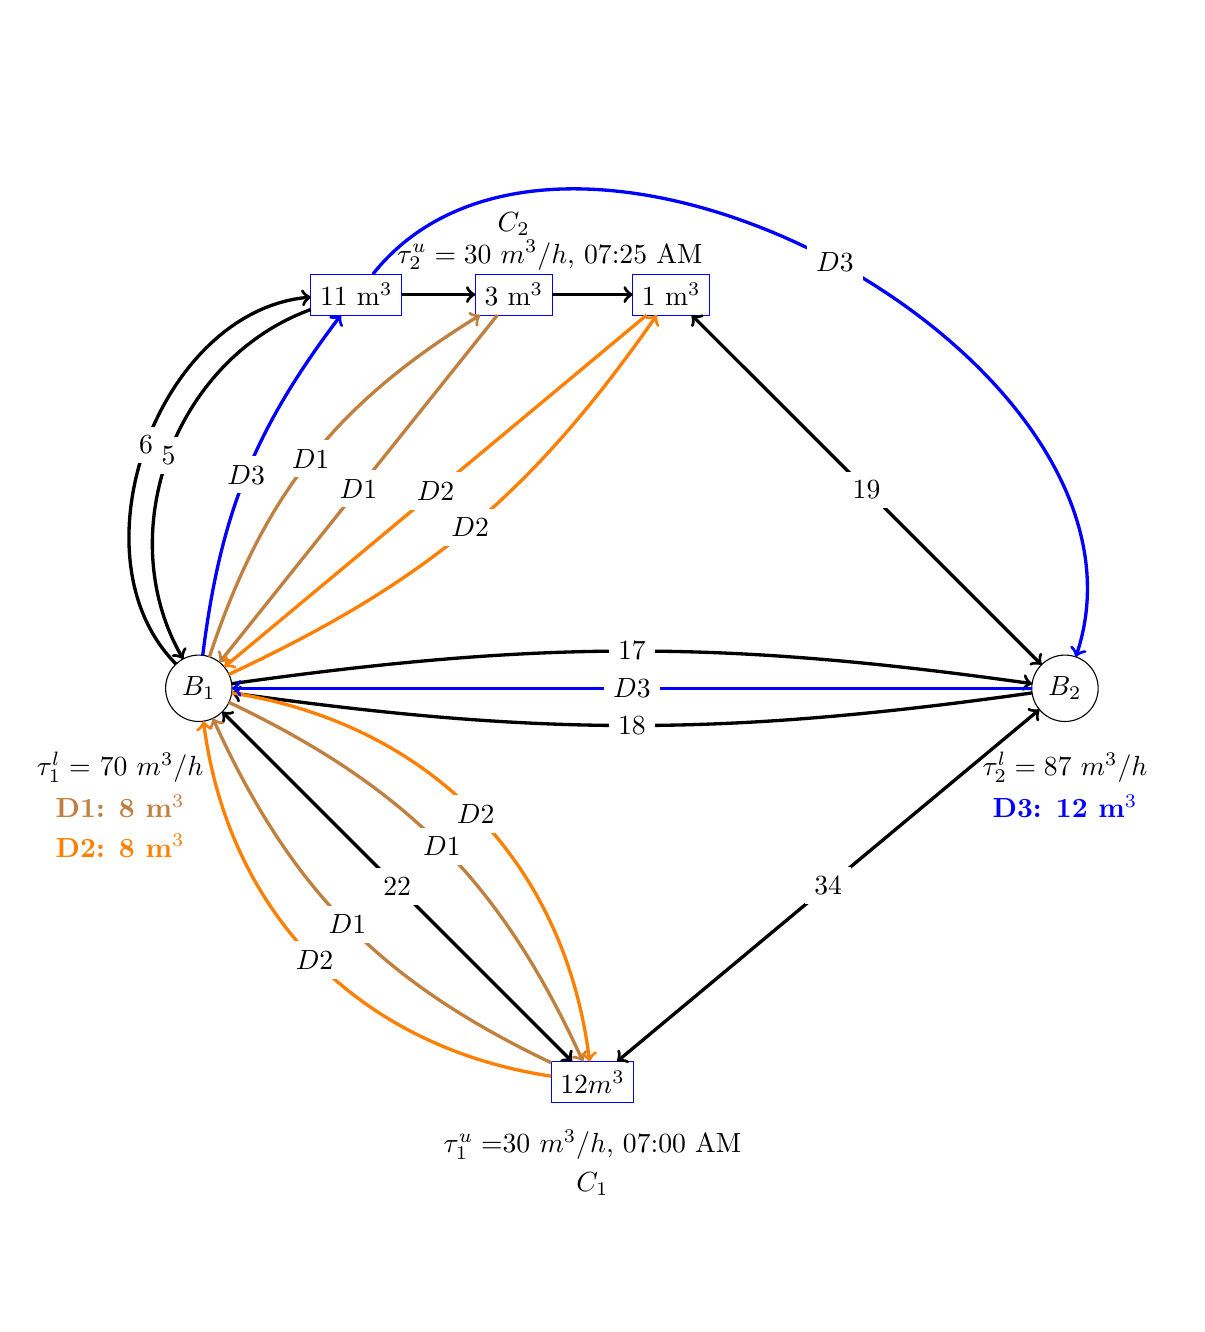
\begin{tikzpicture}
            \SetUpEdge[lw = 1.2pt,
                labelcolor = white,
                % labelstyle = {draw}
            ]
            \tikzstyle{LabelStyle}=[fill=white]

            \SetGraphUnit{5}
            \GraphInit[vstyle=Normal]
            \tikzset{VertexStyle/.style = {shape = circle,text = black,minimum size = 24 pt,draw = black}}
            \Vertex[L={$B_1$}]{D1}
            \tikzset{VertexStyle/.style = {shape = circle,text = black,minimum size = 10 pt,draw = blue}}
            \tikzset{VertexStyle/.style = {shape = rectangle,text = black,minimum size = 10 pt,draw = blue}}
            \Vertex[x=2,y=5,L={11 m$^3$}]{C21}
            \EA[unit=2.0,L={3 m$^3$}](C21){C22}
            \EA[unit=2.0,L={1 m$^3$}](C22){C23}
            \tikzset{VertexStyle/.style = {shape = rectangle,text = black,minimum size = 10 pt,draw = blue}}
            \SOEA[L={$12m^3$}](D1){C1}
            \tikzset{VertexStyle/.style = {shape = circle,text = black,minimum size = 24 pt,draw = black}}
            \SOEA[L={$B_2$}](C23){D2}
            % %  \SetVertexArt
            \tikzset{VertexStyle/.style = {shape = circle,text = black,minimum size = 10 pt}}
            \SO[unit=0.8,L={$\tau^u_1=$30 $m^3/h$, 07:00 AM}](C1){tau1}
            \SO[unit=0.5,L={\textbf{$C_1$} }](tau1){o1}

            \NO[unit=0.9,L={\textbf{$C_2$}}](C22){C2}
            \SOEA[unit=0.4,L={\textcolor{white}{  } $\tau^u_2=30$ $m^3/h$, 07:25 AM}](C2){tau2}

            \tikzset{VertexStyle/.style = {shape = rectangle,text = black,minimum size = 10 pt}}
            \SOWE[unit=1.,L={$\tau^l_1=$ 70 $m^3/h$}](D1){cap1}
            \SO[unit=0.5,L={\textbf{\textcolor{brown}{D1: 8 m$^3$}}}](cap1){driver11}
            \SO[unit=0.5,L={\textbf{\textcolor{orange}{D2: 8 m$^3$}}}](driver11){driver12}
            \SO[unit=1,L={$\tau^l_2= 87$ $m^3/h$}](D2){cap2}
            \SO[unit=0.5,L={\textbf{\textcolor{blue}{D3: 12 m$^3$}}}](cap2){driver2}
            %%%%%%% Edge
            \tikzset{EdgeStyle/.style={->}}
            \Edge[](C21)(C22)
            \Edge[](C22)(C23)
            \tikzset{EdgeStyle/.style={<->,bend left=0}}
            \Edge[label=$22$](D1)(C1)
            \tikzset{EdgeStyle/.style={<->}}
            \Edge[label=$19$](D2)(C23)
            \Edge[label=$34$](D2)(C1)
            \tikzset{EdgeStyle/.style={->}}
            \tikzset{EdgeStyle/.append style = {bend left = 8}}
            \Edge[label=$17$](D1)(D2)
            \Edge[label=$18$](D2)(D1)
            \tikzset{EdgeStyle/.append style = {bend left = 65}}
            \Edge[label=$6$](D1)(C21)
            \tikzset{EdgeStyle/.append style = {bend right = 50}}
            \Edge[label=$5$](C21)(D1)
            \tikzset{EdgeStyle/.style = {->,bend left = 20,draw=brown}}
            \Edge[label=$D1$](D1)(C1)
            \Edge[label=$D1$](C1)(D1)
            \tikzset{EdgeStyle/.style = {->,bend left = 37,draw=orange}}
            \Edge[label=$D2$](C1)(D1)
            \Edge[label=$D2$](D1)(C1)

            \tikzset{EdgeStyle/.style = {->,bend left= 20,draw=brown}}
            \Edge[label=$D1$](D1)(C22)
            \tikzset{EdgeStyle/.style = {->,bend left= 0,draw=brown}}
            \Edge[label=$D1$](C22)(D1)

            \tikzset{EdgeStyle/.style = {->,bend left = 0,draw=orange}}
            \Edge[label=$D2$](C23)(D1)
            \tikzset{EdgeStyle/.style = {->,bend left = -15,draw=orange}}
            \Edge[label=$D2$](D1)(C23)


            \tikzset{EdgeStyle/.style = {->,,draw=blue}}
            \Edge[label=$D3$](D2)(D1)
            \tikzset{EdgeStyle/.style = {->,bend left = 15,draw=blue}}
            \Edge[label=$D3$](D1)(C21)
            \tikzset{EdgeStyle/.style = {->,bend left = 80,draw=blue}}
            \Edge[label=$D3$](C21)(D2)
        \end{tikzpicture}
    \end{adjustbox}
    \vspace*{-10mm}
    % }
    \caption{Solution of an instance with two plants, two construction sites, four orders, and three drivers.}
    \label{fig_Example}

\end{figure}

\begin{figure}[htbp]
    \centering

    \vspace*{-0mm}
    \begin{adjustbox}{max width=0.85\textwidth}
        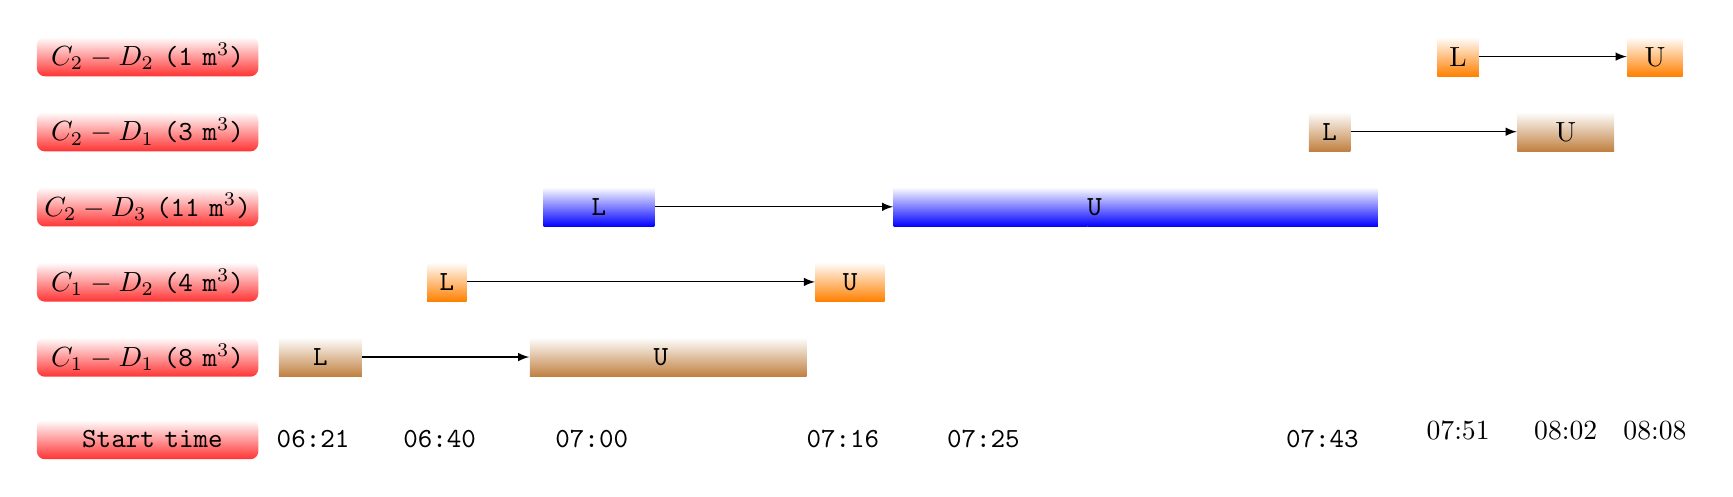
\begin{tikzpicture}[-latex]
            \matrix (chart)
            [
            matrix of nodes, nodes in empty cells,
            column sep      = 0em,
            row sep         = 3ex,
            column 1/.style = {nodes={label}},    column 2/.style = {},       column 3/.style = {nodes={env}},      column 4/.style = {nodes={env}},         column 5/.style = {nodes={env}},         column 6/.style = {nodes={env}},           column 7/.style = {nodes={env}},           column 8/.style = {nodes={env}},           column 9/.style = {nodes={env}},           column 10/.style = {nodes={env}},         column 11/.style = {nodes={env}},           column 12/.style = {nodes={env}},    column 13/.style = {nodes={env}}
            ]
            {
            $C_2-D_2$ (1 m$^3$) &
            &   &   &   &   &   &   &   &   &   &   &   &            |[LC23]| L &            &       &     |[UC23]| U \\
            $C_2-D_1$ (3 m$^3$) &           &      &        &        &           &            &            &
            &
            &
            &
            |[LC21]| L &
            &
            &
            &
            |[UC21]| U &
            \\
            $C_2-D_3$ (11 m$^3$) &
            &
            &
            &
            &
            &
            |[LC22]| L &
            &
            &
            |[UC22]| &
            |[UC22]|U  &
            |[UC221]|  &
            &
            &
            &
            &
            \\
            $C_1-D_2$ (4 m$^3$) &
            &
            &
            &
            |[LC12]| L &
            &
            &
            &
            |[UC12]| U &
            &
            &
            &
            &
            &
            &
            &
            \\
            $C_1-D_1$ (8 m$^3$) &
            &
            |[LC11]| L &
            &
            &
            &
            |[UC11]|U &
            |[UC11]| &
            &
            &
            &
            &
            &
            &
            &
            &
            \\
            \vspace*{-10em}
            Start time &&
            06:21 &
            &
            06:40 &
            &
            07:00 &
            &
            07:16 &  07:25 &
            &
            07:43 &
            &
            07:51 &
            &
            08:02 & 08:08 \\
            };
            % \node[fit={(chart-3-10) (chart-3-12)},style=UC22]{U};
            \draw (chart-5-3) edge (chart-5-7);
            % \draw (chart-5-8.3) edge (chart-2-12);
            \draw  (chart-4-5) edge (chart-4-9);
            % \draw  (chart-4-9) edge (chart-1-14);
            \draw  (chart-3-7) edge (chart-3-10);
            \draw  (chart-2-12) edge (chart-2-16);
            \draw  (chart-1-14) edge (chart-1-17);

        \end{tikzpicture}
    \end{adjustbox}
    \caption{Schedule of the instance of Figure~\ref{fig_Example}.}
    \label{fig:ganttExample}
\end{figure}


\section{Constructive heuristics and GRASP}
\label{grasp_method}

In this section, we present the heuristic approach we implement to solve this variant of the Concrete Delivery Problem. Our method consists of constructing feasible solutions to the CDP with randomized greedy heuristics and iteratively invoking these heuristics in the GRASP metaheuristic. From now on, we represent the scheduling of a delivery node $d$ as the pair  ($L^k_{d}$,$U^k_{d}$) of loading and unloading tasks. $L^k_{d} = \left(b,q_d,v_b,w_b\right)$ indicates that driver $k$ starts loading $q_d$ $m^3$ of RMC at plant $b$ between $\left[v_b,w_b\right]$. $U^k_{d} = \left(k,v_d, w_d\right)$ indicates that driver $k$ serves $d$ between $v_d$ and $w_d$. We then call a solution $ S =\left\lbrace \cup _{1 \leq j \leq |\mathcal{D}|} (L^k_{j}, U^k_{j}), k \in K \right\rbrace$ the set of all loading and unloading tasks performed on a given day.

\subsection{GRASP algorithm }

The GRASP algorithm, proposed by \cite{feo1989probabilistic}, is a two-phase iterative suite consisting of constructive and local search algorithms. In the construction phase, a feasible solution $S$ is generated using a greedy randomized algorithm. Then, a local search algorithm explores the neighborhood of $S$ to identify a local optimum. Algorithm~\ref{alg_grasp} outlines the pseudocode of the GRASP algorithm. To avoid redundant computations, a hash table $H$ is used to ensure that the local search is not applied multiple times to the same solution.  The procedure stops and returns the best overall solution when certain stopping conditions, such as reaching a time limit or a maximum number of iterations, are met. %In our implementation, we also add a path relinking procedure that uses information about previous solutions to improve the search process.

    {\setstretch{1.0}
        {\small
            \begin{algorithm}[hbpt]
                \caption{Pseudo-code of the GRASP algorithm }
                \label{alg_grasp}
                \DontPrintSemicolon
                \LinesNumbered
                \setcounter{AlgoLine}{0}
                % \KwIn{ \textit{H}: List of constructive greedy randomized heuristics }
                \KwIn{ $\phi$: number of iterations before path relinking }
                $S^* \leftarrow \emptyset$    \hspace{2mm} $T \leftarrow \emptyset$       $Cost(S^*) \leftarrow \infty$

                Initialize an empty hash table $H$

                % $counter \leftarrow  0$

                \While{Conditions not met}{

                    $S \leftarrow GreedyRandomizedHeuristic()$

                    \uIf{ $S \notin H$}{
                        $S \leftarrow LocalSearch(S)$

                        Add $S$ to $H$
                    }

                    % $T \leftarrow T \cup \{S\}$


                    \uIf{$Cost(S)< Cost(S^*)$}{
                        $S^* \leftarrow S$
                    }

                    % \uIf{$counter \text{ } mod \text{ } \phi == 0$}{
                    %     $S^* \leftarrow PathRelinking(T)$

                    %     $T \leftarrow \emptyset$
                    % }

                    % $counter \leftarrow counter + 1$

                }

                \KwRet{$S^{*}$}
            \end{algorithm}}
    }

For the construction phase, we have developed two greedy randomized heuristics. The first heuristic, called customer-based insertion, schedules customers one at a time. On the other hand, the second heuristic, called delivery-based insertion, does not necessarily complete the scheduling of one customer before starting to plan another customer's schedule.
% The greedy aspect of GRASP is the creation of the set $RCL$, the probabilistic aspect is the random selection in $RCL$, and the adaptive aspect is the updating of $CL$ and the re-evaluation of the incremental costs.

\subsection{Customer-based insertion heuristic}

The customer-based insertion heuristic builds a solution from scratch by scheduling all of a customer's orders one at a time. As shown in Algorithm~\ref{alg:greedyCustIns}, for each customer, we randomly select the first order to schedule. To schedule an order, we iterate over each of its delivery nodes, find a feasible pair of tasks, and add it to the current solution. For a delivery node $d$, we check if the list of operations $M[d]$ is empty. If it is, for each available driver $k$ we simulate the loading and unloading operations $(L^k_d,U^k_d)$ with the procedure $SimulateVisit$, and if $k$ can serve $d$, we add $k$ to a candidate list $CL$ and $(L^k_d,U^k_d)$ to $M[d]$.

The $SimulateVisit$ procedure takes a partial solution, a delivery node $d$, a driver $k$ and a numeric value $\lambda$ as parameters. Its goal is to find the earliest time when an unloading service can start at $d$ and the best position within the route of $k$. When planning to visit node $d$ of order $o$ and customer $i$ with driver $k$, we first compute his expected delivery time $v_d$ as follows:

$ v_d = \left\{
    \begin{array}{rl}
        a_i + \lambda                                                   & \text{for the first visited node} \\
        w_j + rand(\lambda, \gamma^1), j \in \mathcal{D}_o,  u_{jd}=1   &                                   \\
        w_j + rand(\lambda, \gamma^2), j \notin \mathcal{D}_o, u_{jd}=1 &
    \end{array}
    \right.$

Then we determine the start loading time $v_l$ of the corresponding dock node $l$ by subtracting the travel time, adjustment time, and loading duration from $v_d$. Starting from $v_l$ we check when $k$ will be available at an idle loading bay and adjust $w_l$ accordingly. Changing $w_l$ can cause the cold-joint constraints to be violated, especially for a customer's subsequent deliveries, and thus make the schedule infeasible. Once we have $v_l$, we can check for the best position to insert the visit of $d$ into the route of $k$.

We extract from $CL$ the restricted candidate list ($RCL$) of drivers for whom the cost of visiting $d$ falls within a specified range based on the parameter $\theta$. If $RCL$ is empty and a visit to $d$ cannot be scheduled due to cold-joint constraints, we use the $DelayPreviousDelivery$ procedure to determine if there is a previous delivery of the same order that we can delay the start of service to visit $d$ feasible. This procedure returns the index of the node and $\lambda$, which is the value of the delay. $\lambda$ is also the same parameter given to $SimulateVisit$. If there is such a previous node, we backtrack to it and restart the scheduling.

If $RCL$ is not empty, we select a random driver from it, insert its corresponding load and unload tasks into $S$, and update the remaining quantities for the order and customer demands. The algorithm returns at the end the constructed solution $S$.


    {\setstretch{1}
        %  {\small
        \begin{algorithm}[htpb]
            \caption{Customer-Based insertion algorithm }
            \label{alg:greedyCustIns}
            \DontPrintSemicolon
            \LinesNumbered
            \setcounter{AlgoLine}{0}
            \KwIn{  $S$: empty solution $S$, $K$: vehicles set \hspace{15mm} \\$\Pi$: custom sorted customers list }

            $M \leftarrow \emptyset $ \tcp{List of pair of loading and unloading tasks for all delivery nodes}
            $CL \leftarrow \emptyset$ \tcp{Candidate driver list all delivery nodes}

            \ForEach(customer $i \in \Pi$){}{

            Shuffle $ \mathcal{O}_i$

            \ForEach{order $o_1 \in \mathcal{O}_i$}{

            $\lambda \leftarrow 0$

            \For{ $j=0$ \KwTo $n^{max}_{o_1}-1$    }{

            Delivery $d =\mathcal{D}^j_{o_1}$

            \uIf{$M[d] == \emptyset $}{

            \ForEach{ $k \in K$  }{

            $(L^k_{d}$, $U^k_{d})$ $\leftarrow $ SimulateVisit($S$,$d$,$k$,$\lambda$)

            $Cost(d,k)$ $\leftarrow $ Cost of ($L^k_{d}$, $U^k_{d}$)

            Add $(L^k_{d}, U^k_{d}$) to $M[d]$

            $CL[d] \leftarrow \{k\}$
            }
            }

            $C_{min} \leftarrow min\left\lbrace C(x), \text{ } x \in M[d] \right\rbrace $, $C_{max} \leftarrow max\left\lbrace C(x), \text{ } x \in M[d] \right\rbrace $

            $RCL \leftarrow \left\lbrace k \in CL[d], \text{ } C(d,k) \leq C_{min} + \theta (C_{max}-C_{min}) \right\rbrace $


            \uIf{$RCL == \emptyset $}{

                $(ind,delay)$ = $DelayPreviousDelivery$($S$,$d$)

                \uIf{j is none}{

                    break \tcp{continue with next customer}
                }
                $j \leftarrow ind$, $\lambda \leftarrow delay$

                continue \tcp{backtrack to $ind$ position }

            }
            Select from $RCL$ a random driver $k$ to visit $d$ with load $q^k_d$

            $M[d]\leftarrow M[d] \backslash (L^k_{d}, U^k_{d})$, $CL[d]\leftarrow CL[d] \backslash \{k\} $

            $S \leftarrow S \cup (L^k_{d}$, $U^k_{d})  $

            $q_i \leftarrow q_i-q^k_{d}$;  $q_{o_1} \leftarrow q_{o_1}-q^k_{d}$

            $\lambda \leftarrow 0$

            \uIf {$q_{o_1} \neq 0$ }{
                continue

            }
            \uElseIf{ $q_i \neq 0$}{
                break

            }
            }
            }
            }

            \KwRet{$S$}
        \end{algorithm}
        %  }
    }

Consider the scenario where two customers require their services to start at the same time or within the same time window. In this case, we can either finish scheduling one customer before the other or schedule both simultaneously.  If there are sufficient resources available, either option would be feasible. However, when resources are limited, the customer-based insertion heuristic may leave some customers unscheduled. To address this limitation, we introduce the delivery-based insertion heuristic.

\subsection{Delivery-based insertion heuristic}

The delivery-based insertion heuristic constructs a feasible solution from scratch by scheduling a delivery node one at a time. The pseudocode for this heuristic is outlined in Algorithm~\ref{alg:delbasedIns}. It starts with an empty solution $S$ and initially fills $CL$ with the first delivery of a randomly selected order for each customer. Within each iteration of the $while$ loop, we filter $CL$ to obtain a reduced candidate list $CL'$ of deliveries from a given neighborhood. With this filtering, we can force the algorithm to schedule nodes with certain criteria first, which could be nodes from customers with the same demand, due date, or geographic area. We can also decide whether to schedule customers with the highest (or lowest) demand or the earliest (latest) due date first.

For each delivery $d$ in $CL'$, the algorithm determines the best available driver $k$ and adds the corresponding loading and unloading task $(L^k_d, U^k_d)$ to a list of tasks. This is done using the $SimulateVisit$ procedure described earlier. Next, the algorithm constructs a $RCL$ from the list of tasks. If it is empty, the algorithm proceeds to the next iteration. Otherwise, it randomly selects a pair of tasks from the $RCL$, inserts them into $S$, and updates the remaining order and customer quantities. If an order $o$ is not fulfilled after visiting $d^j_{o}$, we add its next delivery node $d^{j+1}_{o}$ to $CL$.  Otherwise, if the customer has remaining orders, we select the first delivery node $d^{0}_{o'}$ of another randomly selected order $o'$ and add it to $CL$.

    % The greedy aspect of GRASP is the creation of the set $RCL$, the probabilistic aspect is the random selection in $RCL$, and the adaptive aspect is the updating of $CL$ and the re-evaluation of the incremental costs.

    {\setstretch{1}
        %  {\small
        \begin{algorithm}[htb]
            \caption{Delivery-based insertion algorithm }
            \label{alg:delbasedIns}
            \DontPrintSemicolon
            \LinesNumbered
            \setcounter{AlgoLine}{0}
            \KwIn{  $S$: empty solution $S$}

            $CL \leftarrow \emptyset$

            \ForEach(customer i){}{

            Select a random order $o_1 \in \mathcal{O}_i$

            $CL \leftarrow CL \cup \{d^0_{o_1}\}$
            }

            \While{$CL \neq \emptyset$}{

            $CL' \leftarrow \text{Filter (CL)} $

            $Tasks \leftarrow \emptyset $ \tcp{List of loading and unloading tasks}

            \ForEach( $d \in CL'$){}{

                % $C(d) \leftarrow$ incremental cost of inserting $d$

                $Tasks \leftarrow (L^k_d,U^k_d)$ \tcp{$k$ is the best available driver to visit $d$}

            }
            $C_{min} \leftarrow \min\left\lbrace Cost(x), \text{ } x \in Tasks \right\rbrace $, $C_{max} \leftarrow \max\left\lbrace Cost(x), \text{ } x \in Tasks \right\rbrace $

            $RCL \leftarrow \left\lbrace x \in Tasks, \text{ } Cost(x) \leq C_{min} + \theta (C_{max}-C_{min}) \right\rbrace $


            \uIf{$RCL \leftarrow \emptyset$}{
                continue
            }

            Select random operations $(L^k_{d^{j}_o},U^k_{d^{j}_o})$ of customer $i$ (order $o$) from $RCL$

            $ S \leftarrow S \cup (L^k_{{d^{j}_o}}, U^k_{{d^{j}_o}})$


            $q_i \leftarrow q_i-q^k_{d^{j}_o}$;  $q_{o} \leftarrow q_{o}-q^k_{d^{j}_o}$

            \uIf {$q_{o} \neq 0$ }{

                $CL \leftarrow CL \cup \{d^{j+1}_{o}\}$

            }
            \uElseIf{ $q_i \neq 0$}{

                Select another order $o' \in \mathcal{O}_i$

                $CL \leftarrow CL \cup \{d^{0}_{o'}\} $

            }

            Update $CL$
            }
            \KwRet{$S$}
        \end{algorithm}
        %  }
    }

\subsection{Local Search}

After the construction phase, the local search phase iteratively invokes five operators using a first-improvement strategy. The first operator (\textit{Swap Load}) exchanges loads between two deliveries of the same order. The \textit{Swap Driver} operator explores alternative driver assignments by swapping drivers assigned to two delivery nodes. The \textit{Relocate} operator removes a delivery node and places it in a different location. The \textit{Consolidate Load} operator assigns an order request initially split between two drivers to a single driver if the driver's capacity allows. The \textit{Remove and Reschedule} operator selects an unscheduled customer, denoted $i$, within the current solution. It then identifies a set $C$ containing scheduled customers with the same time slot as $i$. All elements of $C$ are removed and rescheduled along with $i$. This local search process continues until no further improvements can be made or a timeout is reached.


% \subsection{Path relinking}

% After the construction and local search steps, it is possible that some customers remain unscheduled in one solution while being accommodated in another. The goal of the path relinking procedure is to use each customer's scheduling information from existing solutions and combine them effectively to construct a solution that schedules all customers. This algorithm iterates through each element of a pool of solutions and attempts to insert each customer's schedule into a newly constructed solution.

\section{Computational experiments}
\label{comp_exp}

In this section, we present and discuss the results of computational experiments conducted using the GRASP heuristic described in section~\ref{grasp_method}. The implementation of the GRASP algorithm is coded in C++. We run our experiments on the benchmark data used in \cite{kinable2014concrete}, and on a new dataset extracted from delivery operations records provided by our industry partner.

\subsection{Generation of instances}
\newcommand{\nbInstance}{36}
The dataset used in this section was obtained from our partner and contains records representing delivery operations from up to 8 production centers for $\nbInstance$ days. From this historical data, we extract information such as daily orders delivered, plant assignments to orders, and the number of available drivers. We created $\nbInstance$ instances from this data, where each instance corresponds to a daily operation. To maintain confidentiality, we have removed the GPS coordinates of customers and plants, but have included two matrices containing the distances and driving times between all plants and customers. An instance contains information such as each driver's capacity, associated batch plant, and shift start time (which we generate). For each customer, we have the due time, the total demand, the number of orders (type of concrete) received, and its index in the time (distance) matrix. For each order, we have its demand and the corresponding production plant. Finally, we have the loading capacity for each plant, and also its index in the time matrix. The name of an instance has the format $C\_k\_n\_o\_z$, where $k$ is the number of available drivers, $n$ is the number of customers, $o$ is the total number of daily orders, and $z$ is the number of plants. The dataset is divided into small, medium, and large sets according to the total number of daily orders. We have summarized the dataset in Table~\ref{tab:instances}. The dataset is available upon request as a contribution to the CDP literature.

\begin{table}[htpb]
    \centering
    \caption{Instances summary}
    \label{tab:instances}
    \small
    \resizebox*{0.8\textwidth}{!}{
        \begin{tabular}{lcccccc}
            \toprule
            {}     & \# & Demand            & \#Order   & \#Client & \#Driver & \#Depot \\
                   &    & (m$^3$)           &           &          &          &         \\
            \midrule
            Small  & 8  & 226.5 - 937.5     & 7 - 14    & 4 - 11   & 13-35    & 1-3     \\
            % \cmidrule{3-7}
            Medium & 14 & 1,160.5 - 2,971.0 & 43 - 98   & 40 - 89  & 76-137   & 6-8     \\
            % \cmidrule{3-7}
            Large  & 14 & 3,078. - 3,953.5  & 107 - 136 & 92 - 127 & 129-150  & 8       \\
            \bottomrule
        \end{tabular}
    }
\end{table}

\subsection{Results for the instances of \cite{kinable2014concrete}}

\cite{kinable2014concrete} provided a benchmark dataset for their variant of the $CDP$. Although their primary objective is to maximize the total load delivered each day, without considering loading operations at a plant and ensuring deliveries within specified time windows, we still use this dataset to analyze and compare the performance of our algorithm under different conditions. Table \ref*{tab:cdp_instances} shows the performance of the GRASP heuristic along with the other methods (CP, MIP, SD-heuristic, and Hybrid) used in \cite{kinable2014concrete}.  For each method, the table shows the average execution time in milliseconds and the corresponding gap between the obtained solution and the upper bound provided by \cite{kinable2014concrete}.

\begin{table}[htbp]
    \centering
    \caption{Performance of the GRASP heuristic on the CDP benchmark instances}
    \label{tab:cdp_instances}
    \scriptsize
    \resizebox{1\textwidth}{!}{
        \begin{tabular}{@{}cccccccccccc@{}}
            \toprule
                                   &     & \multicolumn{2}{c}{CP}     & \multicolumn{2}{c}{MIP}   & \multicolumn{2}{c}{SD-heuristic} & \multicolumn{2}{c}{Hybrid} & \multicolumn{2}{c}{GRASP}                                                            \\ \cmidrule(l){3-10} \cmidrule(l){11-12}
                                   &     & Gap (\%)                   & Time (ms)                 & Gap (\%)                         & Time (ms)                  & Gap (\%)                   & Time (ms) & Gap (\%) & Time (ms) & Gap (\%) & Time (ms) \\ \cmidrule(l){3-10} \cmidrule(l){11-12}
            \multirow{2}{*}{Set A} & Avg & 4.2                        & 197,012                   & 7.3                              & 13,405,798                 & 9.1                        & 23        & 7.0      & 100,765   & 5.7      & 13,186    \\ \cmidrule(l){2-10} \cmidrule(l){11-12}
                                   & Opt & \multicolumn{2}{c}{40/64}  & \multicolumn{2}{c}{37/64} & \multicolumn{2}{c}{30/64}        & \multicolumn{2}{c}{35/64}  & \multicolumn{2}{c}{35/64}                                                            \\ \cmidrule(l){3-10} \cmidrule(l){11-12}
            \multirow{2}{*}{Set B} & Avg & 12.1                       & 357,313                   & -                                & -                          & 16.3                       & 1,331     & -        & -         & 13.8     & 574,983   \\ \cmidrule(l){2-10} \cmidrule(l){11-12}
                                   & Opt & \multicolumn{2}{c}{55/128} & \multicolumn{2}{c}{-}     & \multicolumn{2}{c}{40/128}       & \multicolumn{2}{c}{-}      & \multicolumn{2}{c}{44/128}                                                           \\ \bottomrule
        \end{tabular}
    }
\end{table}

Overall, the GRASP algorithm shows promise in providing near-optimal solutions in a relatively short time for this benchmark of the CDP, making it a suitable candidate for further analysis and real-world application. It outperformed all methods except CP, achieving an average distance of 5.7\% (13.8\%) with a runtime of 13,186 (574,983) milliseconds for Set A (Set B). The SD-heuristic appears to be much faster, but GRASP provides a better balance between solution quality and computation time. It should also be noted that the exact MIP, CP, and Hybrid are initialized with the results of the SD-heuristic.


\subsection{Results for the generated instances}

The computational results of our instances solved with the GRASP heuristic are summarized in the tables below. %The stopping criteria are set to 20,000 iterations or 3600 seconds of running time (unless otherwise specified).
The parameters used in our experiments are listed in Table~\ref*{tab:problem_parameters}.

\begin{table}[hbt]
    \centering
    \caption{Parameters of the real-world instances}
    \label{tab:problem_parameters}
    \small
    \begin{tabularx}{\textwidth}{Xr}
        \toprule
        \multicolumn{1}{c}{Parameter}  &
        \multicolumn{1}{c}{Value} \\ \midrule
 Time window ($\tau^w$)  & 60 min    \\
 Unloading duration ($\tau_c^u$)  & 2 min$/m^3$   \\
 Cleaning duration ($\rho$)    & 10 min  \\
        Adjustment duration ($\alpha$)                                                & 10 min                    \\
        Max travel time ($\Delta$)                                                    & 120 min                   \\
        Min working time ($M_T$)                                                      & 180 min                   \\
        Max working time ($N_T$)                                                      & 480 min                   \\
        Max overtime duration ($O_T$)                                                 & 120 min                   \\
        Max delay between two consecutive deliveries of the same order $\gamma^1$)   & 20 min                    \\
        Max delay between two consecutive deliveries of different orders ($\gamma^2)$ & 25 min                    \\
        Penalty of unfulfilled orders ($\beta_1$)                                     & 10,0000                   \\
        Penalty of first delivery delay ($\beta_2$)                                   & 1,0000                    \\
        Penalty for driver underutilization  ($\beta_3$)                              & 30                        \\
        Driver overtime penalty $ (\beta_4$)                                          & 20                        \\
        \bottomrule
    \end{tabularx}
\end{table}

The table \ref*{tab:all_instances} contains the detailed results for all instances with a stop criterion of 3600 seconds. The table shows the demand of each instance, the average, and the best values of the objective function when solving each instance five times. All daily orders of the small instances are completely served by our algorithm within these five iterations, as shown in column $UQ$, which reports the undelivered quantity. For the medium and large instances, $99.57\%$ and $99.5\%$ of the total demands are delivered. The sum of driver underutilization costs ($DUC$) is high for medium and large instances. This indicates the underutilization of the scheduled fleet. Some drivers are not scheduled at all or work very little. The sum of driver overtime costs ($DOC$) is also high for these instances. This can be explained by the fact that the algorithm prefers to put drivers on overtime rather than use a driver who has to travel to another plant for a delivery, which would increase travel costs ($TC$).

FDD represents the sum of the delays of the first deliveries. In the case of small instances, all but one of the first deliveries are on time. However, for the other instance sets, there is at least one customer with a late first delivery. To provide insight into the actual delay experienced by customers, we report mFDD, which is the maximum delay among all first deliveries. This information reveals that for small instances, the maximum delay ranges between 0 and 35.7 minutes. For medium instances, it varies from 16.8 to 60 minutes, and for large instances, it falls within the range of 56 to 60 minutes.

\begin{table}[htb]
    \centering
    \caption{Results with all instances}
    \label{tab:all_instances}
    \resizebox{\textwidth}{!}{
    \begin{tabular}{llcccccccccccccc}
    \toprule
    &                 &          & \multicolumn{6}{c}{Avg} & \multicolumn{6}{c}{Best}  \\
    \cmidrule(l){4-9} \cmidrule(l){10-16}
     &  & Demand & $TC$ & $UQ$ & $FDD$ & $DUC$ & $DOC$ & \multirow[c]{2}{*}{Z} & $TC$ & $UQ$ & $FDD$ & $mFDD$ & $DUC$ & $DOC$ & \multirow[c]{2}{*}{Z} \\
     &  & ($m^3$) & (min) & ($m^3$) & (min) & (min) & (min) &  & (min) & ($m^3$) & (min) & (min) & (min) & (min) &  \\
    \midrule
    \multirow[c]{8}{*}{Small} & C_13_11_12_1 & 226.5 & 1,243.5 & 0.0 & 0.0 & 10.8 & 0.0 & 1,568.3 & 1,243.5 & 0.0 & 0.0 & 0.0 & 0.0 & 0.0 & 1,243.5 \\
     & C_13_5_8_1 & 267.0 & 745.1 & 0.0 & 0.0 & 0.0 & 0.0 & 745.1 & 745.1 & 0.0 & 0.0 & 0.0 & 0.0 & 0.0 & 745.1 \\
     & C_18_6_11_2 & 333.5 & 753.3 & 0.0 & 0.0 & 145.9 & 0.0 & 5,130.0 & 753.3 & 0.0 & 0.0 & 0.0 & 118.7 & 0.0 & 4,315.1 \\
     & C_15_4_7_2 & 375.0 & 1,015.6 & 0.0 & 0.0 & 148.2 & 150.5 & 8,470.9 & 1,015.4 & 0.0 & 0.0 & 0.0 & 123.4 & 110.3 & 6,924.5 \\
     & C_19_7_8_2 & 388.0 & 1,747.2 & 0.0 & 0.0 & 349.8 & 159.0 & 15,421.6 & 1,781.8 & 0.0 & 0.0 & 0.0 & 186.0 & 0.0 & 7,361.5 \\
     & C_29_10_14_3 & 613.5 & 3,510.1 & 0.0 & 59.5 & 194.6 & 331.9 & 75,488.1 & 3,493.4 & 0.0 & 59.5 & 35.7 & 120.5 & 60.0 & 67,810.4 \\
     & C_31_8_11_3 & 776.0 & 2,314.8 & 0.0 & 0.0 & 804.3 & 640.7 & 39,256.8 & 2,278.2 & 0.0 & 0.0 & 0.0 & 503.5 & 617.0 & 29,722.9 \\
     & C_35_9_10_3 & 937.5 & 4,175.5 & 0.0 & 0.0 & 222.1 & 669.3 & 24,224.7 & 4,163.1 & 0.0 & 0.0 & 0.0 & 243.3 & 570.0 & 22,863.2 \\
     \cmidrule(l){1-16}

    \multirow[c]{14}{*}{Medium} & C_76_40_43_6 & 1,160.5 & 6,055.8 & 0.0 & 49.1 & 3,286.4 & 990.0 & 173,509.5 & 5,990.6 & 0.0 & 33.9 & 25.4 & 3,061.3 & 788.6 & 147,510.1 \\
     & C_104_42_47_8 & 1,565.0 & 8,107.1 & 12.0 & 53.3 & 3,637.1 & 119.4 & 1,372,936.3 & 8,301.9 & 12.0 & 54.3 & 16.8 & 3,200.5 & 140.1 & 1,361,393.1 \\
     & C_94_63_70_7 & 1,746.5 & 13,783.0 & 0.0 & 238.7 & 983.2 & 1,554.6 & 313,077.0 & 13,673.5 & 0.0 & 195.9 & 59.7 & 1,025.2 & 1,407.3 & 268,524.2 \\
     & C_116_67_78_8 & 1,839.5 & 13,456.8 & 0.0 & 132.7 & 1,869.0 & 614.3 & 214,501.3 & 13,484.8 & 0.0 & 98.0 & 22.7 & 1,792.8 & 622.4 & 177,710.8 \\
     & C_116_71_82_8 & 2,060.0 & 11,393.8 & 9.0 & 265.1 & 2,714.8 & 1,054.6 & 1,279,068.9 & 10,793.3 & 9.0 & 242.0 & 41.8 & 3,197.9 & 665.2 & 1,262,000.5 \\
     & C_117_57_70_6 & 2,327.5 & 14,975.0 & 0.0 & 324.1 & 1,005.5 & 1,149.6 & 392,281.0 & 15,303.5 & 0.0 & 295.2 & 54.6 & 659.4 & 1,083.8 & 351,940.4 \\
     & C_137_79_83_7 & 2,425.0 & 17,644.3 & 0.0 & 553.8 & 2,320.4 & 1,993.3 & 680,888.1 & 17,379.3 & 0.0 & 474.0 & 55.7 & 2,964.4 & 2,016.3 & 620,601.6 \\
     & C_127_66_80_8 & 2,512.5 & 14,584.3 & 0.0 & 128.3 & 1,600.0 & 1,451.5 & 219,949.8 & 14,499.2 & 0.0 & 127.5 & 47.3 & 1,390.2 & 1,212.8 & 207,962.2 \\
     & C_128_68_74_7 & 2,595.0 & 18,450.6 & 3.7 & 566.6 & 1,317.5 & 2,706.2 & 1,048,712.1 & 18,261.4 & 0.0 & 473.4 & 56.0 & 1,764.7 & 2,525.6 & 595,143.5 \\
     & C_136_85_97_8 & 2,673.0 & 16,831.6 & 0.0 & 379.9 & 2,702.4 & 2,368.0 & 525,199.5 & 17,241.3 & 0.0 & 323.7 & 50.2 & 2,190.5 & 2,767.1 & 461,973.3 \\
     & C_128_78_85_8 & 2,685.5 & 15,679.8 & 63.0 & 474.5 & 1,399.6 & 2,394.4 & 6,880,077.6 & 15,830.6 & 63.0 & 432.7 & 57.8 & 1,206.8 & 2,272.7 & 6,830,154.3 \\
     & C_131_77_85_8 & 2,893.5 & 16,988.0 & 0.0 & 374.5 & 1,557.9 & 1,996.1 & 478,106.8 & 16,565.6 & 0.0 & 352.1 & 44.6 & 1,624.3 & 1,322.5 & 443,865.0 \\
     & C_137_89_97_7 & 2,939.5 & 21,716.4 & 9.8 & 924.4 & 821.0 & 3,494.4 & 2,020,622.6 & 21,311.3 & 0.0 & 799.5 & 51.8 & 887.3 & 3,486.7 & 917,162.4 \\
     & C_133_84_98_7 & 2,971.0 & 20,435.5 & 46.1 & 1,141.3 & 894.1 & 2,127.8 & 5,841,090.1 & 20,520.4 & 9.0 & 1,411.0 & 59.5 & 705.0 & 1,871.9 & 2,390,157.6 \\
     \cmidrule(l){1-16}
    \multirow[c]{14}{*}{Large} & C_132_98_109_8 & 3,078.5 & 22,994.6 & 0.0 & 465.5 & 496.5 & 3,804.8 & 579,471.0 & 22,712.7 & 0.0 & 351.5 & 56.2 & 803.2 & 4,011.3 & 478,549.4 \\
     & C_129_101_119_8 & 3,229.0 & 17,323.1 & 11.0 & 657.8 & 1,577.6 & 2,375.9 & 1,869,937.5 & 17,311.8 & 11.0 & 598.8 & 58.4 & 1,507.7 & 1,948.1 & 1,800,315.9 \\
     & C_141_114_136_8 & 3,350.5 & 19,891.6 & 39.1 & 1,255.8 & 1,366.2 & 2,251.9 & 5,271,698.5 & 19,556.2 & 18.0 & 1,366.7 & 57.9 & 1,380.0 & 2,695.1 & 3,281,568.6 \\
     & C_140_114_132_8 & 3,401.5 & 21,917.6 & 23.8 & 1,254.1 & 680.1 & 3,389.9 & 3,744,172.5 & 22,590.2 & 17.5 & 1,248.5 & 58.7 & 766.3 & 3,267.6 & 3,109,441.2 \\
     & C_143_101_123_8 & 3,437.5 & 23,477.2 & 0.0 & 677.7 & 955.5 & 4,369.4 & 817,244.5 & 23,806.9 & 0.0 & 617.3 & 56.0 & 1,302.2 & 5,147.9 & 783,123.1 \\
     & C_137_112_129_8 & 3,471.0 & 22,089.2 & 0.0 & 546.6 & 544.8 & 4,187.3 & 668,737.0 & 21,195.2 & 0.0 & 456.6 & 55.0 & 883.9 & 3,532.1 & 574,935.0 \\
     & C_142_114_129_8 & 3,499.5 & 20,678.2 & 35.7 & 1,007.5 & 1,119.7 & 4,133.1 & 4,714,436.9 & 21,243.7 & 21.0 & 907.0 & 59.8 & 1,038.0 & 4,016.6 & 3,139,750.0 \\
     & C_149_98_122_8 & 3,513.0 & 19,859.0 & 28.4 & 1,141.7 & 2,154.6 & 2,649.9 & 4,119,224.3 & 19,602.8 & 21.0 & 859.2 & 55.7 & 2,342.9 & 2,728.2 & 3,103,676.6 \\
     & C_139_98_108_8 & 3,541.0 & 21,060.5 & 0.0 & 966.2 & 684.9 & 3,585.4 & 1,079,477.1 & 21,084.8 & 0.0 & 867.2 & 59.8 & 834.9 & 4,133.9 & 996,046.7 \\
     & C_144_108_122_8 & 3,670.5 & 23,330.4 & 2.0 & 1,123.4 & 536.2 & 3,251.6 & 1,427,866.8 & 22,882.8 & 0.0 & 969.7 & 57.8 & 649.7 & 3,587.1 & 1,083,850.9 \\
     & C_142_92_107_8 & 3,684.5 & 23,179.0 & 0.0 & 578.3 & 384.1 & 4,260.4 & 698,184.4 & 23,610.6 & 0.0 & 449.2 & 59.8 & 315.7 & 4,257.2 & 567,403.7 \\
     & C_138_114_136_8 & 3,739.5 & 23,614.6 & 11.7 & 1,225.1 & 837.4 & 5,668.6 & 2,557,166.5 & 22,859.0 & 7.5 & 1,107.0 & 58.3 & 1,224.2 & 5,078.2 & 2,018,119.1 \\
     & C_150_127_136_8 & 3,946.5 & 24,940.3 & 0.0 & 949.5 & 775.5 & 5,384.3 & 1,105,391.3 & 24,939.2 & 0.0 & 829.0 & 57.1 & 805.9 & 6,166.7 & 1,001,490.6 \\
     & C_148_112_131_8 & 3,953.5 & 24,286.0 & 34.0 & 1,247.8 & 657.0 & 3,009.5 & 4,752,026.9 & 24,221.7 & 24.5 & 1,118.5 & 57.1 & 859.7 & 3,483.3 & 3,688,169.1 \\
    \bottomrule
    \end{tabular}
    }
\end{table}
    
Table \ref{tab_runtime} shows that as the algorithm runtime increases, a higher percentage of deliveries are completed. For small instances, all requests are delivered in less than a minute, while for medium and large instances, 99\% of requests are delivered. 

\begin{table}[htb]
    \centering
    \caption{RMC delivery completion within different runtimes of the GRASP}
    \label{tab_runtime}
    \scriptsize
    \resizebox*{0.7\textwidth}{!}{
    \begin{tabular}{llrrrrr}
    \toprule
     &  & \multicolumn{5}{c}{Runtime (min)} \\
     \cmidrule{3-7}
     &  & 1 & 5 & 10 & 30 & 60 \\
    \midrule
    Small & \%Load & 100.00 & 100.00 & 100.00 & 100.00 & 100.00 \\
    Medium & \%Load & 99.00 & 99.29 & 99.29 & 99.43 & 99.57 \\
    Large & \%Load & 99.00 & 99.21 & 99.36 & 99.43 & 99.50 \\
    \bottomrule
    \end{tabular}
    }
\end{table}
    
Figure \ref*{fig:plants_schedules} provides a visual representation using Gantt charts of the loading and unloading operations for the orders assigned to each plant in instance $C29\_10\_14\_3$. It also shows the different assignments of each driver throughout the day. This instance has three plants, twenty-nine drivers, and ten customers, with two customers having multiple orders. Customer $8$ has two orders ($o_8$,$o_9$) assigned to plant $0$ while customer $9$ has four orders ($o_{10}$ - - $o_{13}$) assigned to plant $2$. All the order requirements are in the table~\ref*{tab:instance_detail}.

\begin{table}[!h]
    \centering
    \caption{Informations of instance $C29\_10\_14\_3$}
    \label{tab:instance_detail}
    \resizebox*{1\textwidth}{!}{
        \begin{tabular}{@{}c|cccccccccccccc@{}}
            \toprule
            Order    & 0     & 1     & 2     & 3     & 4     & 5     & 6     & 7     & 8     & 9     & 10    & 11    & 12    & 13    \\ \midrule
            Customer & 0     & 1     & 2     & 3     & 4     & 5     & 6     & 7     & 8     & 8     & 9     & 9     & 9     & 9     \\
            \midrule
            Demand   & 3.0   & 6.0   & 6.5   & 9.5   & 10.0  & 15.0  & 17.0  & 118.0 & 1.0   & 210.5 & 1.0   & 3.0   & 19.0  & 194.0 \\
            \midrule
            Plant    & 1     & 1     & 1     & 1     & 1     & 1     & 1     & 2     & 0     & 0     & 2     & 2     & 2     & 2     \\
            \midrule
            TW       & 09:00 & 10:00 & 12:00 & 09:15 & 07:00 & 07:00 & 10:30 & 10:00 & 07:00 & 07:00 & 07:25 & 07:25 & 07:25 & 07:25 \\ \bottomrule
        \end{tabular}
    }
\end{table}

We can see that the loading operations for each plant do not overlap, and the unloading operations occur sequentially, one after the other, at each worksite. Plant $0$ is responsible for both orders from customer $8$. In the figure~\ref*{fig:plant0}, order $o_8$ is served before $o_9$, starting at the due time. Each row in the figure represents the pairs of loading and unloading tasks performed by a driver. The number next to a task refers to the order.  Figure~\ref*{fig:plant2} shows how the loading bay is alternately assigned to orders $o_{13}$ and $o_7$ between $10:00$ and $14:00$. Driver $26$ starts his service at plant $0$, serves order $o_9$ four times, and travels to plant $2$ to make the final delivery of order $o_{13}$. Driver $25$ also loads at both plants $0$ and $1$.

We report a $FDD$ of $59.5$ minutes for this solution of instance $C29\_10\_14\_3$. The Gantt chart shows that the $4.5$ customers who need their deliveries at $07:00$ all have a late first delivery. These delays are due to the work schedules of the drivers assigned to Plant 1. These drivers start their shifts at the earliest at $06:05$ and $06:20$, and it takes them $59$ to $63$ minutes to reach the 4 to 5 customers. This finding suggests that the relatively high FDD values in our results may be related to suboptimal scheduling of drivers' hours in our instances.

\begin{figure}[htb]
    \centering
    \begin{subfigure}{0.5\textwidth}
        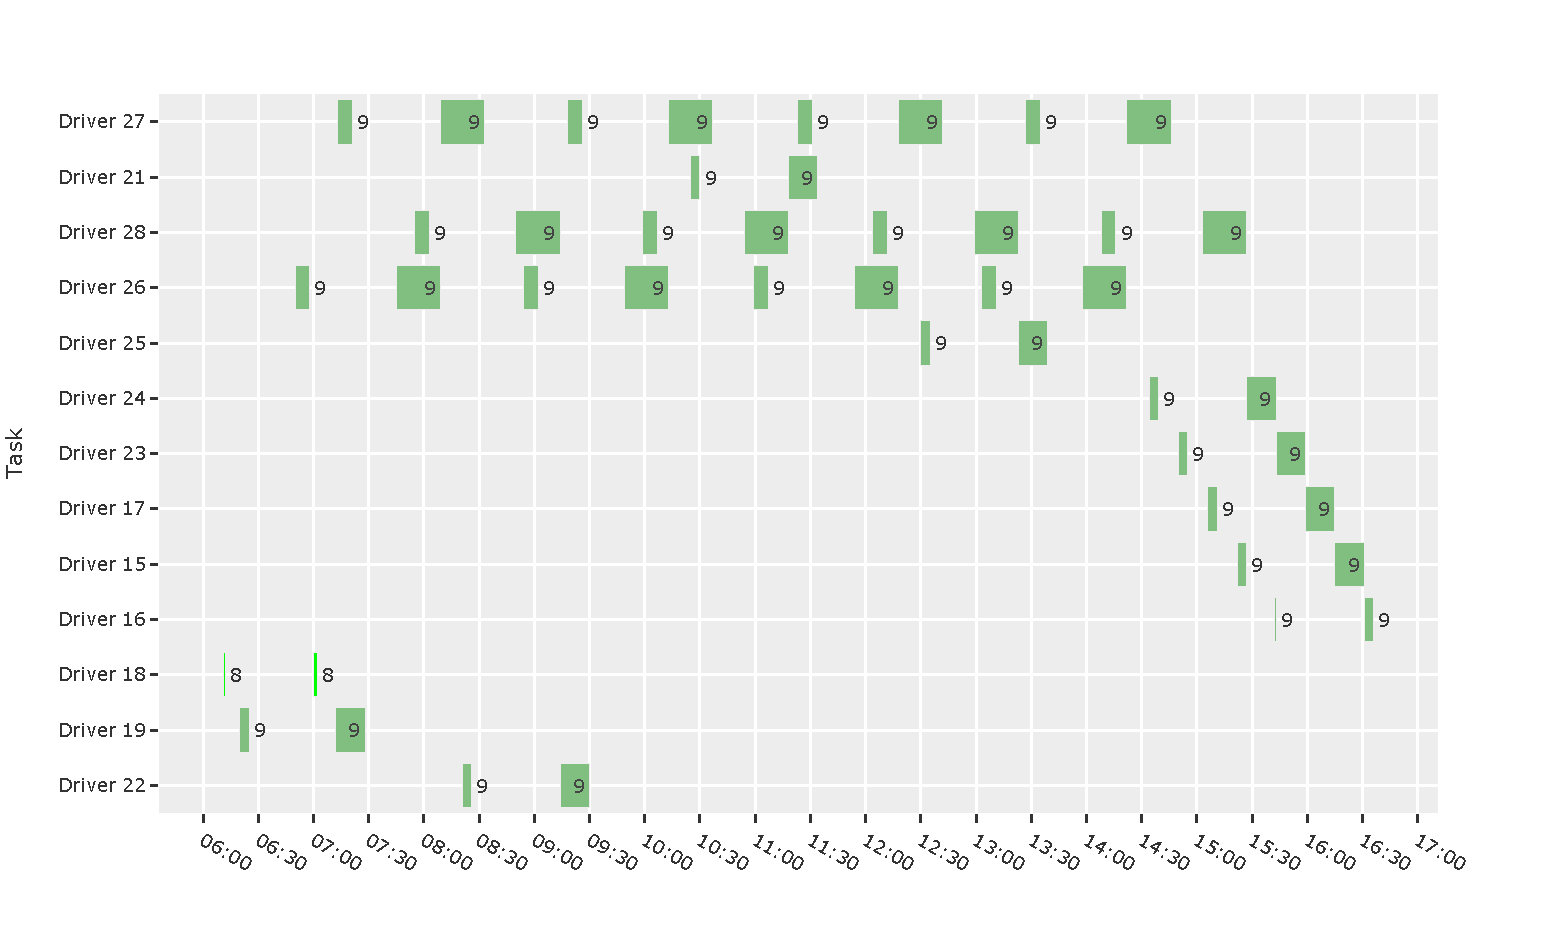
\includegraphics[width=\linewidth]{depot_0.pdf}
        \vspace*{-2em}
        \caption{Scheduling of tasks at plant 0}
        \label{fig:plant0}
    \end{subfigure}%
    \hfill% Horizontal space between the subfigures
    \begin{subfigure}{0.5\textwidth}
        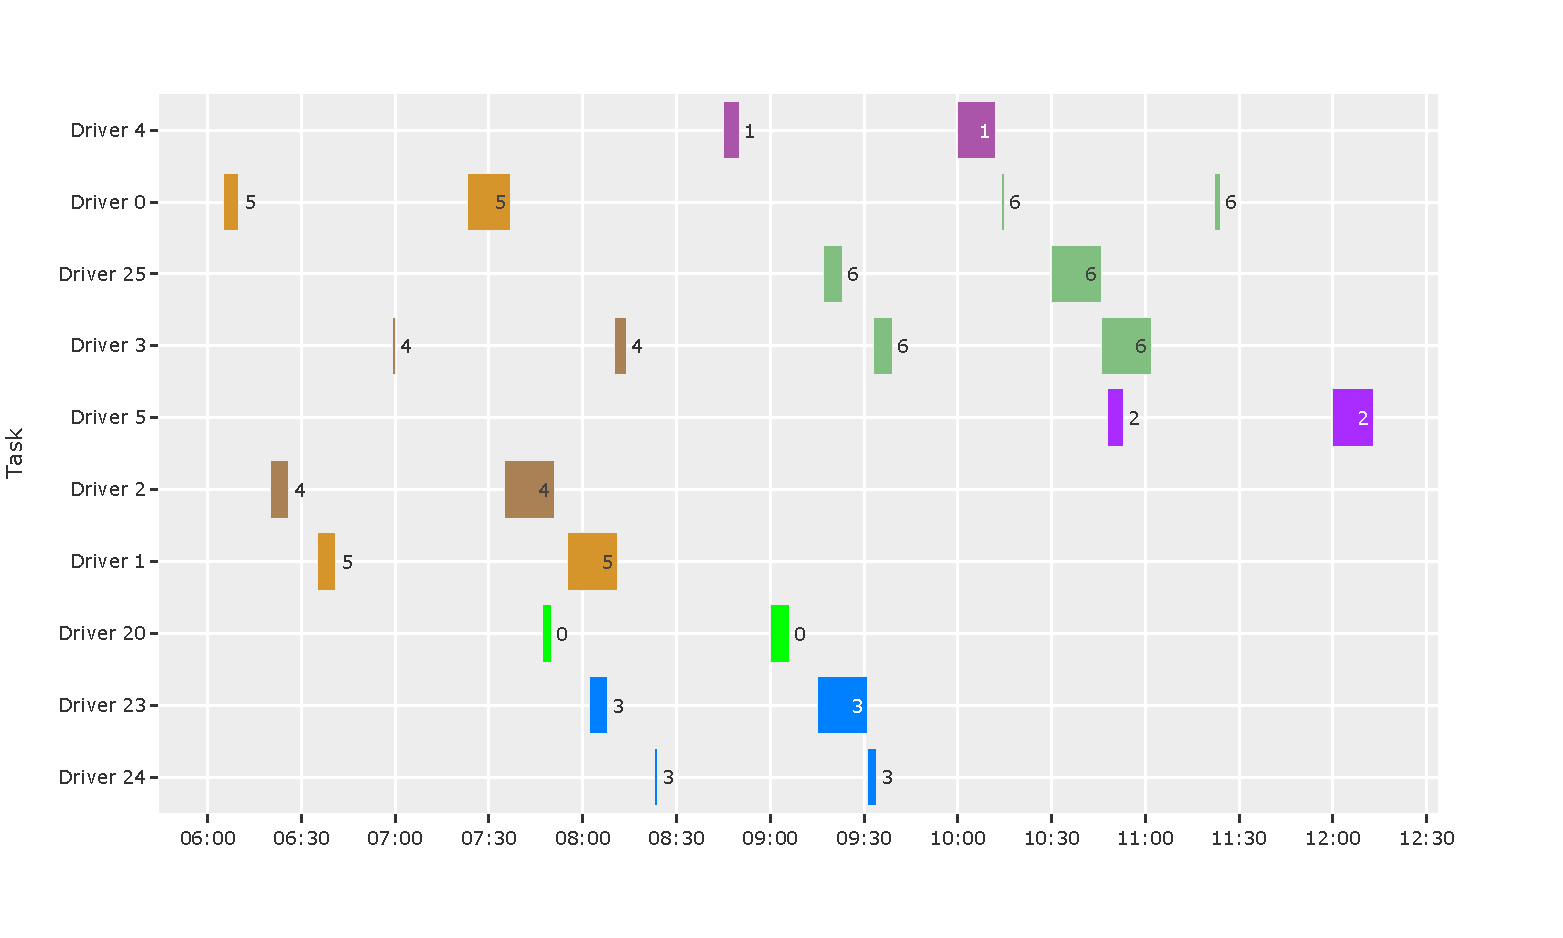
\includegraphics[width=\linewidth]{depot_1.pdf}
        \vspace*{-2em}
        \caption{Scheduling of tasks at plant  1}
        \label{fig:plant1}
    \end{subfigure}
    \vspace*{-1mm}
    \begin{subfigure}{\textwidth}
        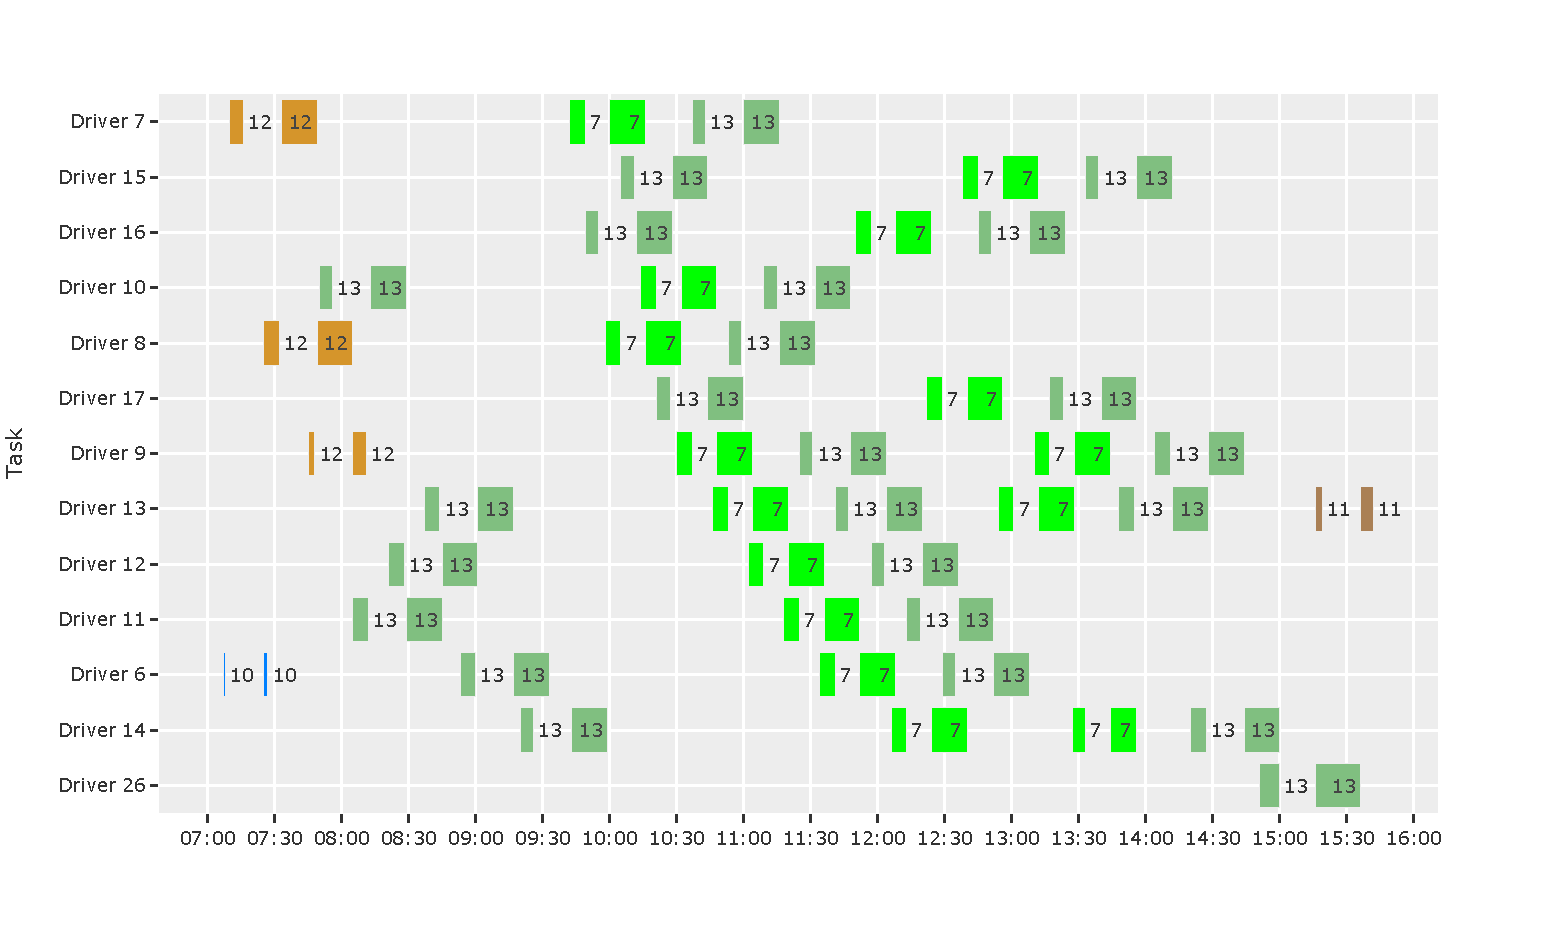
\includegraphics[width=\linewidth]{depot_2.pdf}
        \vspace*{-3em}
        \caption{Scheduling of tasks at plant  2}
        \label{fig:plant2}
    \end{subfigure}

    \caption{Loading and unloading schedules for the plants of instance $C29\_10\_14\_3$}
    \label{fig:plants_schedules}
\end{figure}

The medium instance $C\_104\_42\_47\_8$ has an unserved customer with a demand of 12 $m^3$ and a due time of $07:00$. Upon investigation, we find that even if we have $104$ drivers in this case, the number of drivers who start their shift before t$07:00$ is not enough to serve this customer within the 60-minute window we defined. Thus, the value of $UQ$ that we report in the table~\ref*{tab:all_instances} appears to be optimal given the driver shift schedule given as input to our algorithm. We confirmed this observation by removing the driver start shift and overtime constraints and resolving our instances five more times. All orders are now fully serviced on each run. The table~\ref*{tab:lift_shift_constraints} compares the averages of the results from  the tables \ref*{tab:all_instances} and \ref*{tab:all_instances_no_shift}. We found that for small instances the maximum delay dropped to zero, and for medium (large) instances it was reduced by almost 60\% (40\%) on average. This suggests that when we input a good work schedule, our algorithm works effectively to ensure that all orders are filled and that delays for first deliveries and travel costs are minimized. We can see that the average travel time decreases in all cases except the large one, where the difference is not significant.

\begin{table}[!h]
    \centering
    \small
    \caption{Comparison of the average results with and without shift and overtime constraints}
    \label{tab:lift_shift_constraints}
    \resizebox{0.8\textwidth}{!}{
    \begin{tabular}{lcccccccc}
    \toprule
     & \multicolumn{4}{c}{Default parameters}&\multicolumn{4}{c}{$M_T=0$, $N_T,O_T=\infty$, $H_k=0$} \\
     \cmidrule(l){2-5} \cmidrule(l){6-9}
     & $TC$ & $UQ$ & $FDD$ & $mFDD$ & $TC$ & $UQ$ & $FDD$ & $mFDD$ \\
     & (min) & ($m^3$) & (min) & (min) & (min) & ($m^3$) & (min) & (min) \\
    \midrule
    Small & 1,938.13 & 0.00 & 7.44 & 4.47 & 1,842.97 & 0.00 & 0.00 & 0.00 \\
    Medium & 15,007.28 & 10.26 & 400.45 & 46.31 & 14,879.19 & 0.00 & 74.11 & 17.87 \\
    Large & 22,045.81 & 13.26 & 935.49 & 56.93 & 22,454.09 & 0.00 & 187.51 & 34.76 \\
    \bottomrule
    \end{tabular}
    }
\end{table}
    
\begin{table}[!ht]
    \centering
    \small
    \caption{Results with all instances without shift and overtime constraints}
    \label{tab:all_instances_no_shift}
    \resizebox{\textwidth}{!}{
    \begin{tabular}{llcccccccccc}
    \toprule
     &  & & \multicolumn{4}{c}{Avg}& \multicolumn{4}{c}{Best}\\
     \cmidrule(l){4-7} \cmidrule(l){8-12}
     &  & Demand & $TC$ & $UQ$ & $FDD$ & \multirow[c]{2}{*}{Z} & $TC$ & UQ & $FDD$ & $mFDD$ & \multirow[c]{2}{*}{Z}  \\
     &  & ($m^3$) & (min) & ($m^3$) & (min) &  & (min) & ($m^3$) & (min) & (min) & \\
    \midrule
    \multirow[c]{8}{*}{Small} & C_13_11_12_1 & 226.5 & 1,243.5 & 0.0 & 0.0 & 1,243.5 & 1,243.5 & 0.0 & 0.0 & 0.0 & 1,243.5 \\
     & C_13_5_8_1 & 267.0 & 745.1 & 0.0 & 0.0 & 745.1 & 745.1 & 0.0 & 0.0 & 0.0 & 745.1 \\
     & C_18_6_11_2 & 333.5 & 753.3 & 0.0 & 0.0 & 753.3 & 753.3 & 0.0 & 0.0 & 0.0 & 753.3 \\
     & C_15_4_7_2 & 375.0 & 1,013.7 & 0.0 & 0.0 & 1,013.7 & 1,013.1 & 0.0 & 0.0 & 0.0 & 1,013.1 \\
     & C_19_7_8_2 & 388.0 & 1,661.0 & 0.0 & 0.0 & 1,661.0 & 1,658.2 & 0.0 & 0.0 & 0.0 & 1,658.2 \\
     & C_29_10_14_3 & 613.5 & 3,235.5 & 0.0 & 0.0 & 3,235.5 & 3,198.6 & 0.0 & 0.0 & 0.0 & 3,198.6 \\
     & C_31_8_11_3 & 776.0 & 2,257.6 & 0.0 & 0.0 & 2,257.6 & 2,219.9 & 0.0 & 0.0 & 0.0 & 2,219.9 \\
     & C_35_9_10_3 & 937.5 & 3,834.0 & 0.0 & 0.0 & 3,834.0 & 3,808.8 & 0.0 & 0.0 & 0.0 & 3,808.8 \\
     \cmidrule(l){1-12}
    \multirow[c]{14}{*}{Medium} & C_76_40_43_6 & 1,160.5 & 5,262.4 & 0.0 & 0.0 & 5,262.4 & 5,187.2 & 0.0 & 0.0 & 0.0 & 5,187.2 \\
     & C_104_42_47_8 & 1,565.0 & 8,278.0 & 0.0 & 0.0 & 8,278.0 & 8,209.6 & 0.0 & 0.0 & 0.0 & 8,209.6 \\
     & C_94_63_70_7 & 1,746.5 & 12,730.3 & 0.0 & 0.0 & 12,730.3 & 12,551.9 & 0.0 & 0.0 & 0.0 & 12,551.9 \\
     & C_116_67_78_8 & 1,839.5 & 11,884.4 & 0.0 & 0.0 & 11,884.4 & 11,641.4 & 0.0 & 0.0 & 0.0 & 11,641.4 \\
     & C_116_71_82_8 & 2,060.0 & 10,750.9 & 0.0 & 0.0 & 10,750.9 & 10,697.1 & 0.0 & 0.0 & 0.0 & 10,697.1 \\
     & C_117_57_70_6 & 2,327.5 & 14,547.0 & 0.0 & 25.8 & 40,380.4 & 14,746.8 & 0.0 & 16.1 & 9.1 & 30,816.0 \\
     & C_137_79_83_7 & 2,425.0 & 17,822.4 & 0.0 & 120.0 & 137,840.9 & 17,982.5 & 0.0 & 92.0 & 17.6 & 110,023.4 \\
     & C_127_66_80_8 & 2,512.5 & 13,622.2 & 0.0 & 0.0 & 13,622.2 & 13,565.0 & 0.0 & 0.0 & 0.0 & 13,565.0 \\
     & C_128_68_74_7 & 2,595.0 & 18,641.7 & 0.0 & 74.1 & 92,744.7 & 18,554.8 & 0.0 & 43.4 & 19.0 & 61,987.5 \\
     & C_136_85_97_8 & 2,673.0 & 17,336.3 & 0.0 & 51.8 & 69,145.9 & 17,610.5 & 0.0 & 23.1 & 16.3 & 40,731.6 \\
     & C_128_78_85_8 & 2,685.5 & 16,781.2 & 0.0 & 55.5 & 72,294.4 & 16,658.5 & 0.0 & 39.4 & 12.5 & 56,076.4 \\
     & C_131_77_85_8 & 2,893.5 & 17,789.1 & 0.0 & 22.0 & 39,787.5 & 16,923.5 & 0.0 & 0.0 & 0.0 & 16,923.5 \\
     & C_137_89_97_7 & 2,939.5 & 21,831.7 & 0.0 & 214.2 & 236,037.5 & 22,630.7 & 0.0 & 157.1 & 48.5 & 179,691.7 \\
     & C_133_84_98_7 & 2,971.0 & 21,031.1 & 0.0 & 474.0 & 495,073.6 & 21,179.3 & 0.0 & 359.8 & 59.8 & 380,980.3 \\
     \cmidrule(l){1-12}
     \multirow[c]{14}{*}{Large} & C_132_98_109_8 & 3,078.5 & 22,272.3 & 0.0 & 7.2 & 29,438.3 & 23,294.5 & 0.0 & 4.0 & 1.8 & 27,252.8 \\
     & C_129_101_119_8 & 3,229.0 & 18,473.8 & 0.0 & 41.6 & 60,111.3 & 18,595.2 & 0.0 & 28.0 & 15.7 & 46,551.2 \\
     & C_141_114_136_8 & 3,350.5 & 21,237.4 & 0.0 & 136.7 & 157,923.2 & 20,762.9 & 0.0 & 110.7 & 18.6 & 131,504.9 \\
     & C_140_114_132_8 & 3,401.5 & 22,518.4 & 0.0 & 174.0 & 196,489.2 & 22,537.0 & 0.0 & 64.8 & 10.6 & 87,390.4 \\
     & C_143_101_123_8 & 3,437.5 & 23,807.5 & 0.0 & 39.1 & 62,917.8 & 23,249.3 & 0.0 & 30.2 & 13.8 & 53,413.3 \\
     & C_137_112_129_8 & 3,471.0 & 22,457.5 & 0.0 & 121.0 & 143,439.3 & 21,878.2 & 0.0 & 27.9 & 7.5 & 49,772.5 \\
     & C_142_114_129_8 & 3,499.5 & 21,574.4 & 0.0 & 362.8 & 384,413.2 & 22,591.1 & 0.0 & 221.0 & 52.9 & 243,564.1 \\
     & C_149_98_122_8 & 3,513.0 & 20,918.7 & 0.0 & 150.6 & 171,499.5 & 19,503.4 & 0.0 & 94.1 & 28.6 & 113,643.5 \\
     & C_139_98_108_8 & 3,541.0 & 21,548.1 & 0.0 & 271.5 & 293,062.8 & 22,008.3 & 0.0 & 239.9 & 47.4 & 261,921.3 \\
     & C_144_108_122_8 & 3,670.5 & 23,604.0 & 0.0 & 169.2 & 192,821.5 & 23,200.9 & 0.0 & 125.9 & 42.5 & 149,122.9 \\
     & C_142_92_107_8 & 3,684.5 & 21,279.5 & 0.0 & 83.8 & 105,084.6 & 21,244.2 & 0.0 & 36.4 & 14.4 & 57,641.8 \\
     & C_138_114_136_8 & 3,739.5 & 24,385.3 & 0.0 & 109.8 & 134,180.9 & 25,218.0 & 0.0 & 71.7 & 15.8 & 96,877.5 \\
     & C_150_127_136_8 & 3,946.5 & 24,434.2 & 0.0 & 391.0 & 415,476.7 & 24,732.2 & 0.0 & 292.5 & 52.8 & 317,191.2 \\
     & C_148_112_131_8 & 3,953.5 & 25,846.2 & 0.0 & 566.8 & 592,677.4 & 26,245.8 & 0.0 & 383.8 & 52.7 & 410,087.8 \\
    \bottomrule
    \end{tabular}
    }
\end{table}
    
\subsection{Sensitivity analyses}

In this section, we analyze the effect on the solution when we change some parameters of our problem and how some components of the objective function influence each other.

\subsubsection{Influence of the maximum time delay $\gamma^1$}

We ran additional tests with different values of $\gamma^1$, varying between 5 and 25 minutes, with no shifts or overtime constraints on the drivers. The influence of the value of the maximum time delay between two consecutive deliveries of the same order is shown in figure~\ref*{fig:gamma1_influence}. For small instances, all customers are served on time regardless of the value of $\gamma^1$. For medium (large) instances, all customers are served with $\gamma^1$ starting at 15 (20) minutes. The delay of initial delivery decreases as $\gamma^1$ increases. These results confirm the fact that when $\gamma^1$ is high, plants have more flexibility to delay current deliveries to make room for new ones or to make customers wait until drivers are available. Increasing the maximum delay from 10 to 20 minutes reduces the first delivery delay by over 50\% for the medium and large cases. The average delivery time does not change significantly regardless of the value of $\gamma^1$.

\begin{figure}[!h]
    \centering
    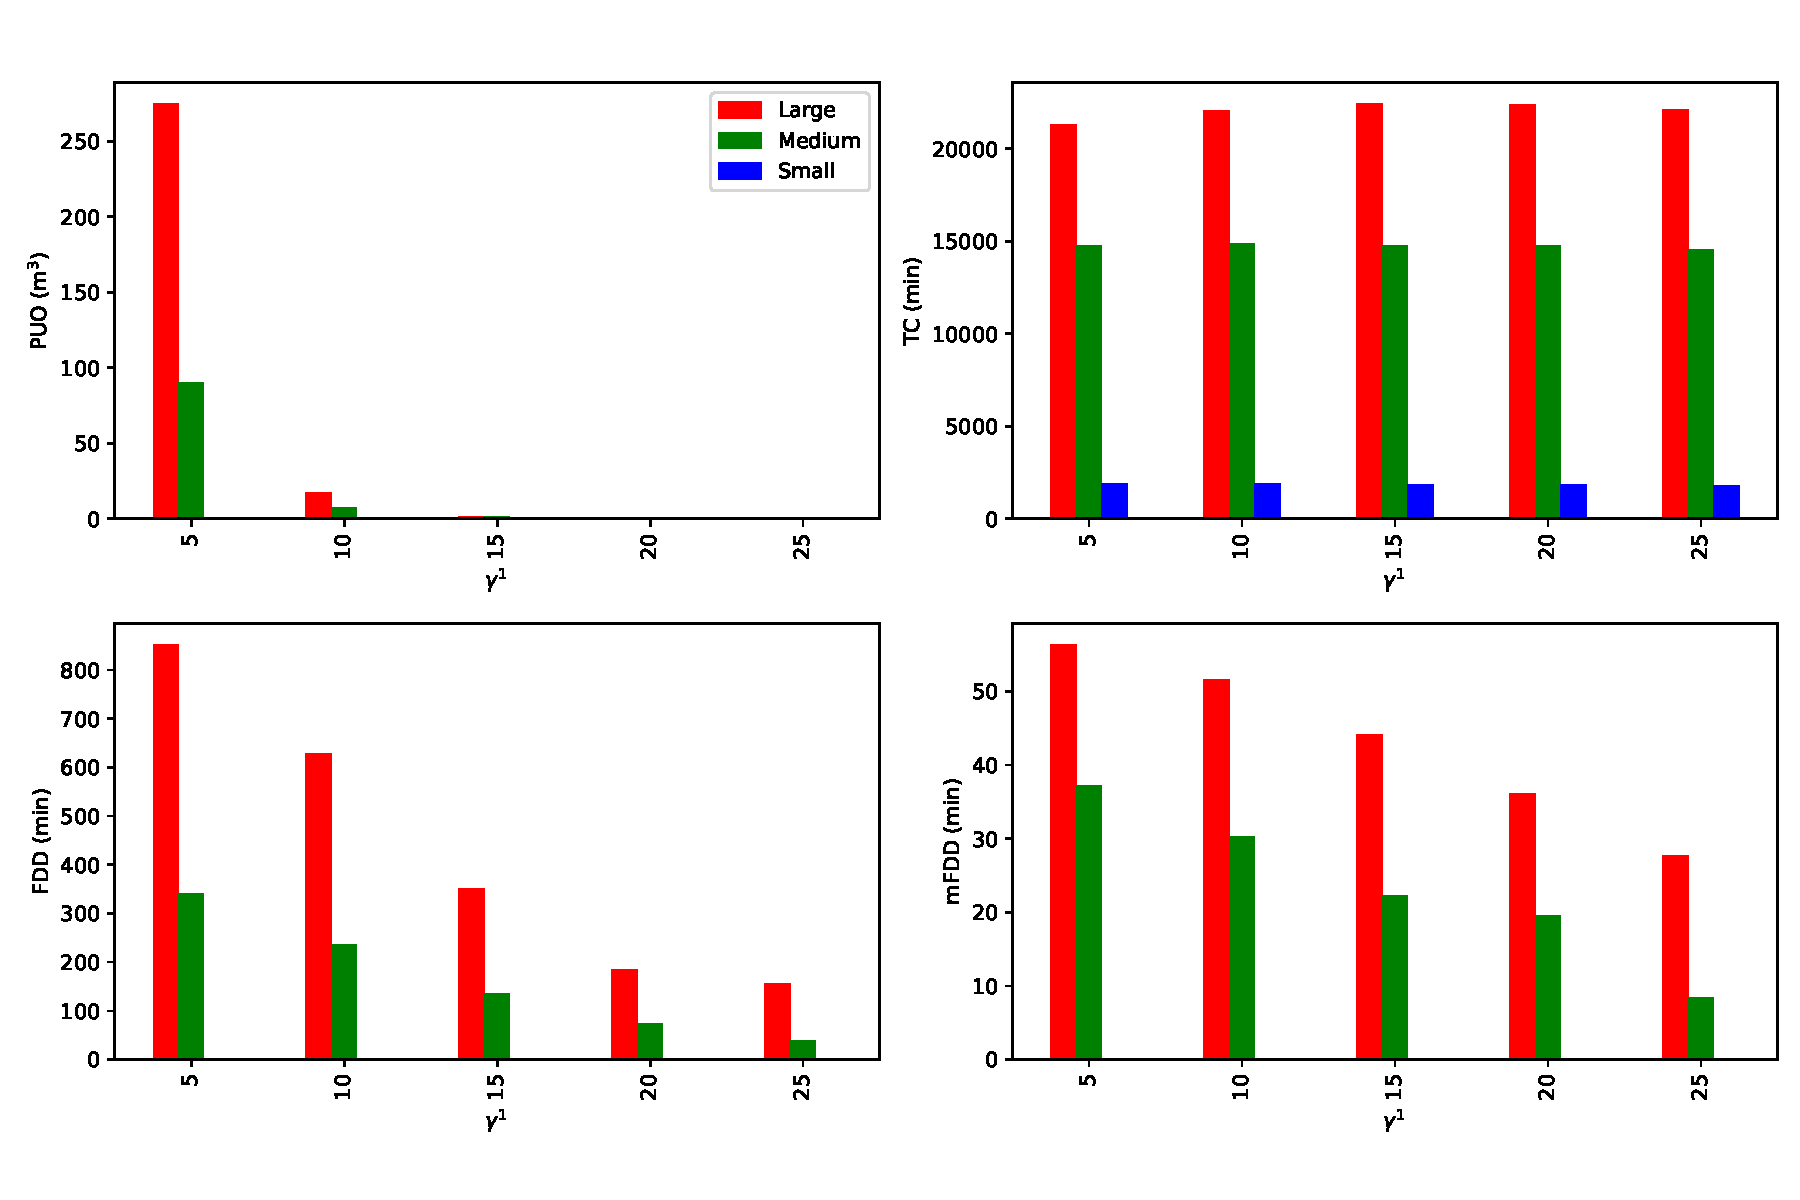
\includegraphics[width=1\textwidth]{gamma1.pdf}
    \small
    \caption{Influence of the maximum time delay ($\gamma^1$) between consecutive deliveries of the same order. }
    \label{fig:gamma1_influence}
\end{figure}

\subsubsection{Trade-off of the objective function components}

We ran five tests on our dataset and obtained two solutions per instance: one that prioritizes the shortest travel time and another that seeks the smallest first delivery delay. Figure~\ref*{fig:trade_off} visually represents the trade-off between travel time and first delivery delay for these solutions. It is clear that as the first delivery delay decreases, the travel time increases, and conversely when the travel time is minimized, the first delivery delay tends to be longer. This result is expected because drivers assigned to a plant often need to travel to another plant to ensure that the first delivery remains on schedule. This trade-off highlights the challenge decision-makers face in finding the right balance between minimizing operational costs and meeting customer satisfaction.

\begin{figure}[!h]
    \centering
    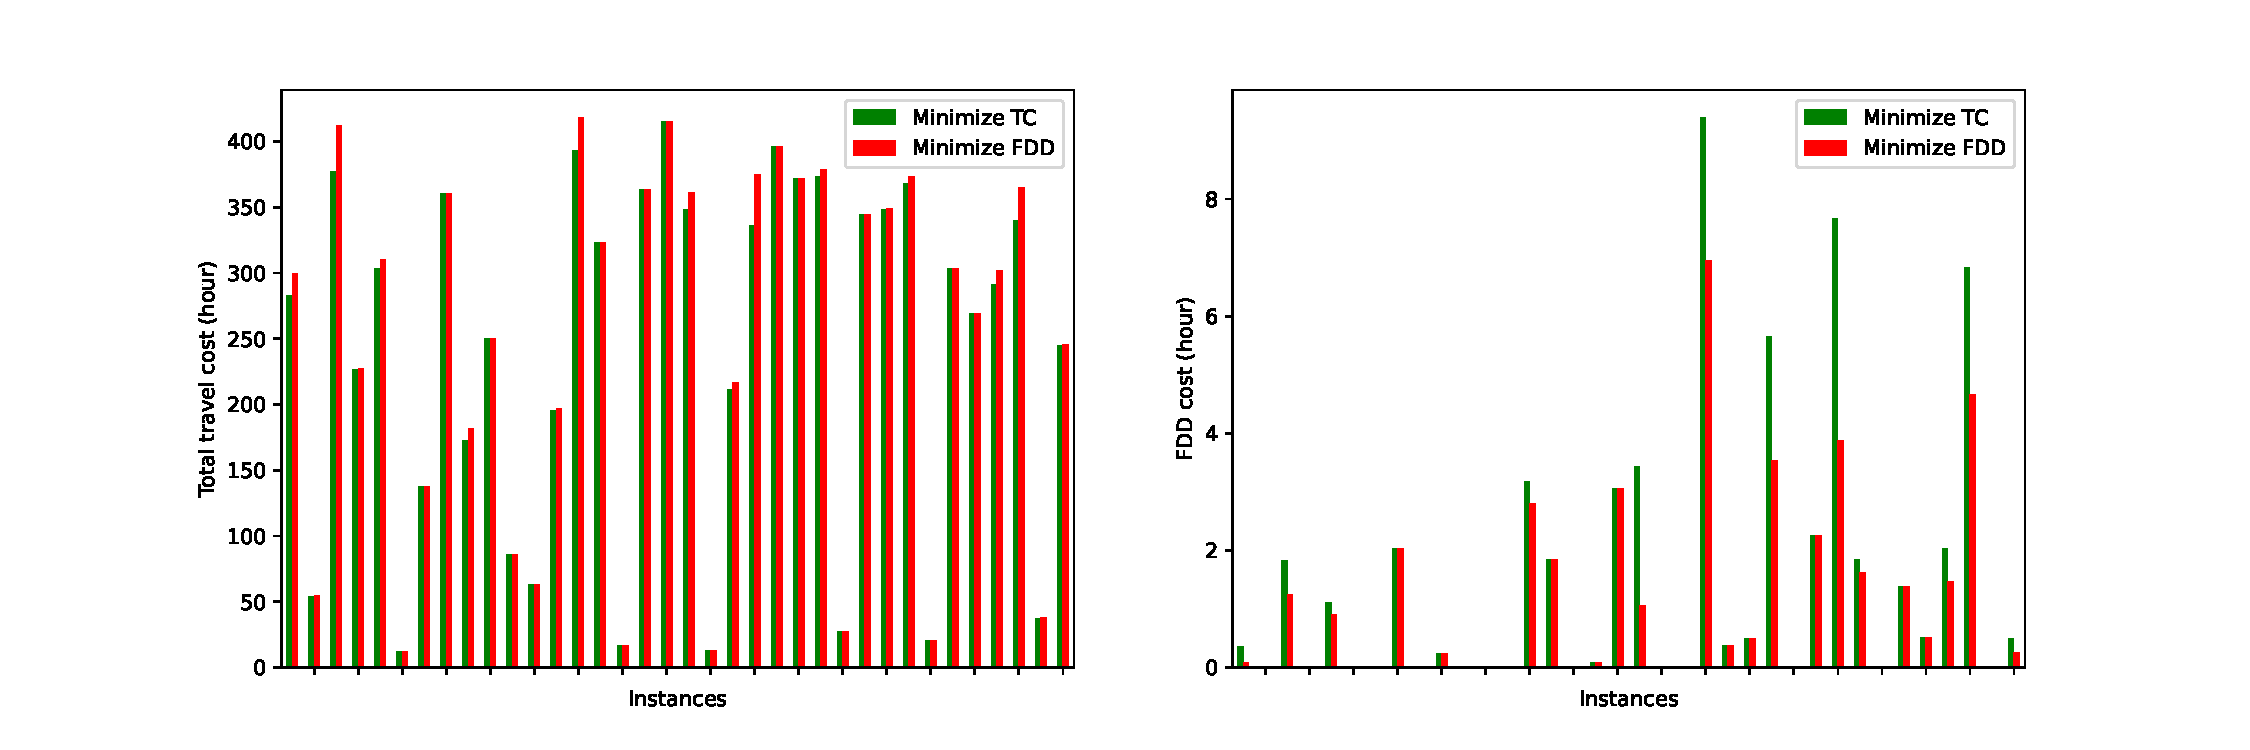
\includegraphics[width=1\textwidth]{Trav_FDD.pdf}
    \small
    \caption{Trade-off between minimizing travel cost VS minimizing first delivery delay }
    \label{fig:trade_off}
\end{figure}

\section{Conclusion}
\label{concl}

In this paper, we investigated a variant of the concrete delivery problem, where customers can order different types of concrete from different production centers, which must be delivered at the same time. To solve this problem, we introduced a mathematical model and a heuristic solution based on Greedy Randomized Adaptive Search. Our analysis, using a dataset derived from our partner's historical data, demonstrated the effectiveness of our algorithm in making good decisions within a reasonable time. Furthermore, our model incorporates constraints related to working hours, making our heuristic a valuable tool for designing weekly schedules for company drivers. Our GRASP algorithm performed exceptionally well on \cite{kinable2014concrete} datasets, indicating its reliability. For future work, it would be interesting to address datasets with different unloading times at construction sites or to explore different scenarios regarding the number of simultaneous deliveries and the maximum time between two consecutive deliveries at a construction site. We can also study the problem using a stochastic or robust methodology to account for the uncertainty of the parameters in a real-world setting. As a contribution to the literature on CDP, we provide a mathematical formulation for our variant, contribute a dataset, and demonstrate the application of GRASP to solve both our problem and the one studied by \cite{kinable2014concrete}.
\vspace{0.1in}

\vspace{1.5cm} \noindent \textbf{Acknowledgments}

Financial support for this work was provided by the Canadian Natural Sciences and Engineering Research Council (NSERC) under grants 2015-04893 and 2019-00094. This support is gratefully acknowledged.


\bibliographystyle{plainnat}
\bibliography{References}


\end{document}